% !TEX root = ..\main.tex
\chapter{Experiments}\label{ch:Experiments}
In this section, we describe the experiments conducted with the dependency model created in this thesis, as well as the PoC. For each of the experiments, we explain the goal, the setup, the results, and finally, we discuss the results and the conclusions extracted from these.

\section{Experiment 1: Comparison}\label{sec:Exp1}
The goal of this experiment is to validate the implementation in the PoC. We compare against the results of the study \textit{"A Comprehensive Study of Bloated Dependencies in the Maven Ecosystem"} by Soto-Valero et al. \cite{soto2020comprehensive}. In this work, a byte-code analysis is performed on Maven Artifacts to detect which of these artifacts' dependencies are \textit{bloated}, which we refer to as \textit{unused}. Although the PoC created in this thesis does not perform the same kind of analysis, we consider that a dependency is \textit{unused} if all the model's metrics detects no usage.

\subsection{Experimental setup}
Soto-Valero et al. perform a qualitative analysis, in which they analyze 31 libraries available as Maven artifacts. If unused dependencies are found during the analysis, a \textit{Pull Request} is made to the \textit{GitHub} repository of the artifact in which the unused dependencies are deleted from the \textit{pom} file.

With the information in the paper, we collect the \textit{GroupId} and \textit{ArtifactId} of the 31 artifacts. Out of the 31, 2 could not be found in the \textit{Maven Repository Central}. For the other 29, the \textit{version} to use in the experiment is determined by finding the last version released before the experiment by Soto-Valero et al. was conducted --- November of 2019.

Of the 29 artifacts, the PoC could not use 13 because either the artifact itself or some dependency could not be downloaded from \textit{Maven Central}. Therefore, we have a set of 16 libraries to analyze and compare the results with the results obtained by Soto-Valero et al. Table \ref{table:comparison-artifacts} contains the identifiers of the artifacts used in this experiment.

\begin{table}[ht!]
    \begin{center}
    \begin{tabular}{|l|l|l|}
    \hline
    Group Id              & Artifact Id                     & Version       \\
    \hline
    org.mybatis           &	mybatis	                        & 3.5.3         \\
    org.apache.flink      & flink-core                      & 1.9.1         \\
    com.puppycrawl.tools  & checkstyle                      & 8.27          \\
    com.google.auto       & auto-common                     & 0.10          \\
    edu.stanford.nlp      & stanford-corenlp                & 3.9.2         \\
    com.squareup.moshi    & moshi-kotlin                    & 1.9.2         \\
    org.neo4j             & neo4j-collections               & 3.5.13        \\
    org.asynchttpclient   & async-http-client               & 2.10.4        \\
    org.alluxio           & alluxio-core-transport          & 2.1.0         \\
    com.github.javaparser & javaparser-symbol-solver-logic  & 3.15.5        \\
    io.undertow           & undertow-benchmarks             & 2.0.27.Final  \\
    org.teavm             & teavm-core                      & 0.6.1         \\
    com.github.jknack     & handlebars-markdown             & 4.1.2         \\
    ma.glasnost.orika     & orika-eclipse-tools             & 1.5.4         \\
    fr.inria.gforge.spoon & spoon-core                      & 8.0.0         \\
    org.jacop             & jacop                           & 4.7.0         \\
    \hline
    \end{tabular}
    \end{center}
    \caption{Identifiers of the Maven artifacts used for comparison}
    \label{table:comparison-artifacts}
\end{table}

The first idea was to create a request that computed the comparison automatically. However, finding why the results were not the same, in most cases, needed manual checking and research. That is why the analysis of the libraries in Table \ref{table:comparison-artifacts} has been executed one by one, and the comparison has been made manually.

\subsection{Results}

The results obtained from the comparison with the data from Soto-Valero et al. \cite{soto2020comprehensive} is done in two parts: if all the libraries found as unused in the paper are also found as unused by the tool, and if all the other libraries are found as used. For the first part, there are several cases:

\begin{itemize}
  \item \textbf{Correct:} All the dependencies detected as unused in the paper are also detected as unused by the PoC.
  \item \textbf{Testing:} At least one of the unused dependencies is a testing dependency, and therefore it is not detected by the PoC.
  \item \textbf{Parent:} At least one of the unused dependencies is from a parent module, and it does not appear in the artifact's tree.
  \item \textbf{Used:} At least one of the unused dependencies is found as used by the PoC.
\end{itemize}

The cases that can happen for the rest of the libraries, the ones that are found as used by Soto-Valero et al. are listed below:

\begin{itemize}
  \item \textbf{Correct:} All the used dependencies, according to the paper, are also used according to the tool.
  \item \textbf{Shaded:} At least one dependency is detected as unused because it is shaded within the jar file of the client library in the building process.
  \item \textbf{Testing:} At least one dependency is found as unused since it is only used for testing, but not marked with scope \textit{testing}.
  \item \textbf{Unused:} At least one dependency found as used by the paper is unused in the tool's analysis.
\end{itemize}

In Table \ref{table:comparison-results}, there are the results for each one of the client libraries used in the experiment.

\begin{table}[ht!]
\begin{center}
\begin{tabular}{|l|l|l|}
\hline
\textbf{Library} & \textbf{Unused in paper} & \textbf{Used in paper} \\ \hline
org.mybatis:mybatis:3.5.3                                   & Testing       & Shaded        \\ \hline
org.apache.flink:flink-core:1.9.1                           & Testing       & Unused          \\ \hline
com.puppycrawl.tools:checkstyle:8.27                        & Testing       & Correct         \\ \hline
com.google.auto:auto-common:0.10                            & Testing       & Unused          \\ \hline
edu.stanford.nlp:stanford-corenlp:3.9.2                     & Correct       & Unused          \\ \hline
com.squareup.moshi:moshi-kotlin:1.9.2                       & Correct       & Correct         \\ \hline
org.neo4j:neo4j-collections:3.5.13                          & Correct       & Unused          \\ \hline
org.asynchttpclient:async-http-client:2.10.4                & Used          & Shaded        \\ \hline
org.alluxio:alluxio-core-transport:2.1.0                    & Correct       & Unused          \\ \hline
com.github.javaparser:javaparser-symbol-solver-logic:3.15.5 & Correct       & Correct         \\ \hline
io.undertow:undertow-benchmarks:2.0.27.Final                & Parent        & Correct         \\ \hline
org.teavm:teavm-core:0.6.1                                  & Parent        & Correct         \\ \hline
com.github.jknack:handlebars-markdown:4.1.2                 & Correct       & Unused          \\ \hline
ma.glasnost.orika:orika-eclipse-tools:1.5.4                 & Testing, Used & Correct         \\ \hline
fr.inria.gforge.spoon:spoon-core:8.0.0                      & Used          & Correct         \\ \hline
org.jacop:jacop:4.7.0                                       & Correct       & Testing, Unused \\ \hline
\end{tabular}
\end{center}
\caption{Results of the comparison with Soto-Valero et al. \cite{soto2020comprehensive}}
\label{table:comparison-results}
\end{table}

\subsection{Discussion}
To evaluate the results of this experiment, we will discuss the meaning of the different cases to detect unused dependencies. There are 9 cases in which the unused dependencies were not correctly detected. Out of these 9, 4 can completely be fixed, if the tool could also analyze the tests defined in the client library. This could be fixed by doing source-code analysis including the testing, instead of bytecode analysis. Also, the 2 cases in which the dependencies are inherited from the parent, and the algorithm used to resolve the dependencies does not include them. Finally, there are 3 cases in which there is at least one dependency which according to the paper should be unused, and it was detected used by the PoC. Therefore, the PoC implementation is overestimating in certain measure the usage of the dependencies.

Next, we take a look at the detection of used dependencies. There are 9 cases in which at least one of the dependencies that were supposed to be used has no usage detected. Two of these cases are due to the dependencies being shaded within the client library's jar during the build process. Also, one case includes a dependency used for testing. These scenarios could be fixed by doing source-code analysis, since the dependencies would not be shaded yet, and the tests could be included in the analysis. Finally, the other 7 cases include dependencies detected as unused, according to the paper by Soto-Valero et al. \cite{soto2020comprehensive}. Therefore, there are some false negatives, which could be related to the way we defined an unused dependency: based on the metrics of the model. It is possible that there are still some types of connections not detected by the tool (e.g., reflection constructs). In some other cases it could happen that it is a very specific type of library, the usage of which cannot be detected on the code. For example, we researched the server libraries of these cases, and it includes a case in which the dependency is related to the compilation of the project. Another case involves a client library in which the part that uses the dependency is not shipped with Maven, and therefore it cannot be detected in the jar file. Finally, there are some empty dependencies - have no classes. A next step could be to investigate what are these libraries used for, and how to detect it.

\begin{finding}
	The scope of the PoC has limited the analysis in some cases such as testing and shaded dependencies. This could be fixed by either including the tests in the jar files, or doing source-code analysis instead.
	\label{find:source-code-analysis}
\end{finding}

\paragraph{Threats to validity}

\section{Experiment 2: Coupling metrics significance}\label{sec:experiment2}

The goal of this experiment is to validate if the coupling metrics designed in the model, namely \texttt{MIC}, \texttt{AC}, \texttt{TMIC}, and \texttt{TAC}, are a good indicator of the usage of the dependencies by the clients. As a partial validation of the metrics' significance, we compare it with the results gathered from the usage metrics. We want to know how often a dependency is used, either by using classes or methods, and it is detected as uncoupled by the coupling metrics. This way, we know if there are many cases in which a dependency is only used with a type of connection other than method invocation or field declaration.

\paragraph{Data collection}
The original idea was to measure real-world data about how the clients update the dependencies and their impact on the code. We could then have seen the correlation of this impact with the degree of dependency measured with the coupling metrics. Different approaches were taken to obtain real-world data.

First, we tried to find GitHub commits in which there had been an update of a dependency. However, the search engine in GitHub does not allow to filter the results by the language of the commit. Therefore, most of the results obtained were not useful. Also, most of the updates are only patches, which require only a bump in the version number of the declared dependency.

Based on these findings, the second approach we took was to look for updates that contained breaking changes. To find the libraries that had these types of changes and versions, we used the \textit{Maven Dependency Dataset} \cite{Raemaekers2013}. Raemaekers et al. used this dataset to analyze the use of semantic versioning and the possible impact of breaking changes \cite{Raemaekers2017}. It is possible to query this dataset to obtain libraries with breaking changes, with version numbers and other libraries that depended on these. However, we need to find the commit of the client library in which the update containing a breaking change was made, and it is not always possible. We considered some of the requirements to be able to analyze a dependency with the PoC. For instance, we need all the dependencies of the client library available in Maven, and testing dependencies cannot be used since they are not analyzed by the tool. Considering all these requirements, obtaining enough data for the experiment from the \textit{Maven Dependency Dataset} had to be done manually.

Next, we contacted the first author of the paper \textit{"Why and How Java Developers Break APIs"} \cite{Brito2018}, which mines GitHub repositories to find possible breaking changes in APIs, to obtain the dataset of breaking changes created based on their findings. Brito, the author, shared the dataset with us. The dataset includes 24 commits containing breaking changes, which correspond to 19 different libraries. Out of the 25 commits, 12 are from Gradle libraries instead of Maven and cannot be used with the PoC. Besides, we could not find four of the commits in GitHub, and two others correspond to testing libraries, which are out of the scope of the analysis performed by the PoC. Therefore, there were only six breaking changes left, for which three the Maven artifact that these belong to had no dependants for which to do the analysis. The last three have only one dependant, and therefore is not possible to compare the impact of the breaking changes.

Finally, we tried to manually search for deprecated libraries and other libraries that used them — however, similar problems where encountered. Finding commits which replaced a deprecated dependency and the client library and all the dependencies are available in \textit{Maven Central Repository}, was a laborious manual task that eventually gave no results.

\subsection{Experimental set up}
In this experiment, we calculated the coupling and coverage metrics of the model, for a set of Maven libraries (see list of libraries in Appendix \ref{appendix:data-set}), to compare the results between the two types of metrics.To run this experiment, we prepared a new request in the API of the PoC. The request has to contain a path to a \textit{.txt} file (tab-delimited). The file has to contain three columns (with headers): \textit{Group Id}, \textit{Artifact Id}, and \textit{version}. For each one of the rows, the metrics are calculated for each of the dependencies. The result of each of the analyses is processed, summarizing all the analyses with the following information:

\begin{itemize}
  \item \textbf{Total number of dependencies:} Number of dependencies of all the analyzed client libraries, including both direct and indirect.
  \item \textbf{Times coupling metrics were not enough:} Number of dependencies for which all the coupling metrics had value zero, but there where methods and classes found reachable by the usage metrics.
  \item \textbf{Times MIC/TMIC were not enough:} Number of times in which there was usage found, but MIC (or TMIC in the case of transitive dependencies) had value zero.
  \item \textbf{Times AC/TAC were not enough:} Number of times in which there was usage found, but MIC (or TMIC in the case of transitive dependencies) had value zero.
  \item \textbf{List server libraries coupling metrics not enough:} The list of \textit{GroupId}, \textit{ArtifactId}, and \textit{version} of the server libraries for which all the coupling metrics were not enough to indicate if there is usage or not.
  \item \textbf{List server libraries MIC/TMIC not enough:} The list of \textit{GroupId}, \textit{ArtifactId}, and \textit{version} of the server libraries for which the metrics \texttt{MIC} and \texttt{TMIC} were not enough to indicate if there is usage or not.
  \item \textbf{List server libraries AC/TAC not enough:} The list of \textit{GroupId}, \textit{ArtifactId}, and \textit{version} of the server libraries for which the metrics \texttt{AC} and \texttt{TAC} were not enough to indicate if there is usage or not.
\end{itemize}

As can be seen, in addition to the number of times that a dependency was used and it was not detected by the metrics (or at least by one of them), the list of server libraries of these dependencies is also stored. This way, it is possible to analyze which types of libraries are those, and why the coupling metrics are not enough to detect their usage.

\blankl
The experiment was run with a file containing 67 client libraries from the \textit{Maven Central Repository}.  We selected the client libraries to use for this experiment with the following criteria. First, we used the same libraries as in the comparison experiment (see Section \ref{sec:Exp1}), but using the last version of each library. We decided to reuse these libraries because the criteria used to select these libraries by Soto-Valero et al. \cite{soto2020comprehensive} is aligned with the needs of this experiment, and are listed below:

\begin{itemize}
  \item The library is relevant - has more than 100 stars on GitHub.
  \item The library can be built successfully with Maven.
  \item Has been developed recently - in the case of Soto-Valero et al., at least October 2019.
  \item The library has at least one dependency declared.
  \item It is indicated how to create a pull request.
\end{itemize}

Although some of the items of the list are not explicitly required for our experiment. We need that the library can be built and is available in Maven as well as that it has at least one relevant dependency (compile scope). Therefore, the libraries in this set are a good fit for the experiment.

To analyze more client libraries and, therefore, more dependencies, we extended the list of libraries. First, we visited the popular libraries list of the \textit{Maven Central Repository} \footnote{\url{https://mvnrepository.com/popular}}. Also, we queried the dataset generated by Harrand et al. \cite{Harrand2019} with the 99 most popular libraries from Maven, according to the number of clients these have. For each of the libraries, we selected the last version available in Maven and filtered the resulting list according to the following criteria:

\begin{itemize}
  \item The artifact of the last version of the library should have at least one dependency with scope compile.
  \item The artifact and all its dependencies can be obtained from the \textit{Maven Central Repository}.
\end{itemize}

\subsection{Results}

The summary of the results of this experiment is shown in Table \ref{table:summary-significance}. We can see the total number of analyzed dependencies, the number of dependencies for which the coverage metrics have found usage, and the coupling metrics have not. The last two rows show the number of dependencies which have more than 0\% coverage, and no coupling has been found by the metrics \texttt{MIC}/\texttt{TMIC} and \texttt{AC}/\texttt{TAC} respectively.

\begin{table}[ht!]
\begin{center}
\begin{tabular}{l|l}
  \hline
  Analyzed dependencies   & 699 \\\hline
  Metrics are not enough  & 35  \\\hline
  MIC/TMIC are not enough & 40  \\\hline
  AC/TAC are not enough   & 147 \\\hline
\end{tabular}
\end{center}
\caption{Summary of the significance experiment}
\label{table:summary-significance}
\end{table}

The server libraries for which usage was found by the coverage metrics but not by the coupling metrics can be found in Table \ref{table:significance-coupling}. The first two columns of this table are the \textit{group id}, and the \textit{artifact id} of the server libraries. Only by looking at the libraries' names, one can see that some of them are libraries that contain \texttt{annotations}. We have checked the content of all the libraries to find out which include only \texttt{annotations}. The result of this search can be seen in the last column of Table \ref{table:significance-coupling}.

\begin{table}[ht!]
\begin{center}
\begin{tabular}{|l|l|l|}
\hline
\textbf{Group Id} & \textbf{Artifact Id} & \textbf{Type} \\
\hline
com.fasterxml.jackson.core  & jackson-annotations             & Annotations \\\hline
com.github.javaparser       & javaparser-symbol-solver-model  & Other       \\\hline
com.google.code.findbugs    & findbugs-annotations            & Annotations \\\hline
com.google.code.findbugs    & jsr305                          & Annotations \\\hline
com.google.errorprone       & error\_prone\_annotations       & Annotations \\\hline
com.google.j2objc           & j2objc-annotations              & Annotations \\\hline
org.apache.flink            & flink-annotations               & Annotations \\\hline
io.grpc                     & grpc-context                    & Other       \\\hline
io.netty                    & netty-codec-socks               & Other       \\\hline
jakarta.activation          & jakarta.activation-api          & Other       \\\hline
org.apiguardian             & apiguardian-api                 & Annotations \\\hline
org.codehaus.mojo           & animal-sniffer-annotations      & Annotations \\\hline
org.codehaus.plexus         & plexus-component-annotations    & Annotations \\\hline
org.codehaus.woodstox       & stax2-api                       & Other       \\\hline
org.glassfish.jaxb          & jaxb-core                       & Other       \\\hline
org.jetbrains               & annotations                     & Annotations \\\hline
org.joda                    & joda-convert                    & Other       \\\hline
org.junit.jupiter           & junit-jupiter-api               & Other       \\\hline
org.neo4j                   & annotations                     & Annotations \\\hline
org.yaml                    & snakeyaml                       & Other       \\\hline
\end{tabular}
\end{center}
\caption{List of the server libraries for which the coupling metrics were not enough to indicate usage}
\label{table:significance-coupling}
\end{table}

\subsection{Discussion}

Based on the results shown in Table \ref{table:summary-significance}, we can see that the combination of the two types of coupling metrics allows us to detect used dependencies in 664/699 of the cases. In addition, the metrics \texttt{MIC} and \texttt{TMIC} alone, detect 659/699 of the cases. This means that \texttt{AC} and \texttt{TAC} are only really needed in 5 of these dependencies. However, this only talks about whether or not the metrics can define whether a dependency is used or not at all, which was not the goal of this thesis. Therefore, \texttt{AC} and \texttt{TAC} are also necessary to consider the type of coupling measured by this metric.

Nevertheless, if we compare the number of times that \texttt{AC}/\texttt{TAC} are not able to detect whether a dependency is used or not, with the times that the same happens with \texttt{MIC}/\texttt{TMIC}, we can conclude that:

\begin{finding}
	Method invocation is enough to detect dependency usage in more cases than Field declaration. Therefore, it is a more significant metric.
	\label{find:significance-mic}
\end{finding}

This is in line with the intuition that method invocation is the most significant type of connection. Generally, if there is an object of a particular class type in the code, at some point, a method call will be done on this object. However, an object can exist in the code through mechanisms other than field declaration (e.g., return type of a method call, or a variable).

Nevertheless, since there are cases in which the combination of both types of metrics was not enough, it indicates that there are some other types of connections to be considered and measured. Given that half of the server libraries used but not detected by the coupling metrics contain annotations, creating a metric to measure the coupling created by annotations would improve these results.

\begin{finding}
	A metric to measure coupling created by the use of annotations would improve the precision of the model. The usage of annotations is sometimes the only type of connection between a client and a server library.
	\label{find:significance-annotations}
\end{finding}

During the process of this thesis, it was intended to create this type of coupling metric. However, it is not a trivial problem for transitive dependencies. In the coupling metrics defined in this thesis, only one type of connection is considered throughout the whole dependency tree. For example, in the dependency tree in Figure \ref{fig:annotation-dependencies}, the client library uses direct dependency through a connection other than annotations. Then, the \textit{non-annotation server library} uses some annotation from the \textit{annotation server library}. Iterating the dependency tree through annotations connection would still not detect the usage of the transitive dependency.

\begin{figure}[ht!]
\begin{center}
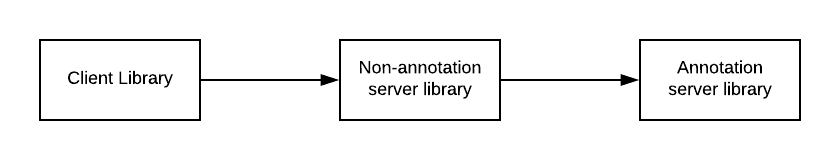
\includegraphics[width=\textwidth]{figures/Transitivity-Annotations.png}
\caption{Example dependency tree involving annotations}
\label{fig:annotation-dependencies}
\end{center}
\end{figure}

\section{Experiment 3: Sensitivity Analysis}
As explained before, we have not been able to obtain the real-world data to understand what the impact of the transitive dependencies is, or can be, and correlate it with our transitive coupling metrics \texttt{TMIC}, and \texttt{TAC}. Therefore, we cannot derive an actual value of the \textit{propagation factor} for these two metrics. Instead, we conduct a sensitivity analysis of the \textit{propagation factor} on these two metrics.

A \textit{Sensitivity Analysis} consists of analyzing how much the output of a model depends on an input variable \cite{Iooss2016}. In this case, the input variable is the \textit{propagation factor}, and the output is the value of the metrics.

\subsection{Experimental set up}

To run this analysis, we have set up a new request in the API of the PoC. This request receives a list of Maven artifacts in a \textit{.txt} file (tab-delimited). The file includes three columns, containing for each artifact, the following information: \textit{group id}, \textit{artifact id}, and \textit{version}.

The first step is to run the dependency model's calculation for each of the dependencies of the artifacts. Then, for each one of the transitive dependencies with coupling, we run the sensitivity analysis. Since the \textit{propagation factor} is a value in the range $(0,1]$, we calculate the value of the metrics incrementing the propagation factor by $0.01$ from $0.01$ to $1$.

We run this experiment with a randomly selected subset of the libraries used for the significance experiment. Then, out of the set of dependencies that can be used for the sensitivity analysis, we select a representative subset of $15$ dependencies. This subset is chosen to have dependencies with different distances, and values measured at each distance. The dependencies used for the sensitivity analysis can be found in Table \ref{table:sensitivity-dependencies}.

\begin{table}[ht!]
\begin{center}
\begin{tabularx}{\textwidth}{|c|X|X|}
\hline
\# &\textbf{Client library} & \textbf{Server library} \\ \hline
1 & org.asynchttpclient async-http-client 2.12.1 & io.netty netty-common 4.1.48.Final \\ \hline
2 & org.asynchttpclient async-http-client 2.12.1 & io.netty netty-buffer 4.1.48.Final \\ \hline
3 & org.easymock easymock 4.2 & org.hamcrest hamcrest-core 1.3 \\ \hline
4 & org.apache.maven maven-project 3.0-alpha-2 & org.codehaus.plexus plexus-classworlds 1.3 \\ \hline
5 & org.springframework.boot\newline spring-boot-autoconfigure 2.3.4.RELEASE & org.springframework\newline spring-core  5.2.9.RELEASE \\ \hline
6 & org.springframework.boot\newline spring-boot-autoconfigure 2.3.4.RELEASE & org.springframework\newline spring-jcl  5.2.9.RELEASE \\ \hline
7 & org.springframework.boot\newline spring-boot-autoconfigure 2.3.4.RELEASE & org.springframework\newline spring-beans  5.2.9.RELEASE \\ \hline
8 & org.eclipse.jetty jetty-server 11.0.0.beta1 & org.eclipse.jetty jetty-util 11.0.0.beta1 \\ \hline
9 & org.asynchttpclient async-http-client 2.12.1 & log4j log4j 1.2.17 \\ \hline
10 & org.alluxio alluxio-core-transport 2.3.0 & com.google.protobuf protobuf-javalite 3.11.0 \\ \hline
11 & fr.inria.gforge.spoon spoon-core 8.2.0 & org.eclipse.platform org.eclipse.osgi 3.16.0 \\ \hline
12 & fr.inria.gforge.spoon spoon-core 8.2.0 & org.eclipse.platform org.eclipse.equinox.preferences 3.8.0 \\ \hline
13 & fr.inria.gforge.spoon spoon-core 8.2.0 & org.eclipse.platform\newline org.eclipse.equinox.common 3.13.0 \\ \hline
14 & com.puppycrawl.tools checkstyle 8.36.2 & log4j log4j 1.2.17 \\ \hline
15 & com.puppycrawl.tools checkstyle 8.36.2 & org.apache.geronimo.specs\newline geronimo-jms 1.1\_spec\_1.0 \\ \hline
\end{tabularx}
\end{center}
\caption{Sensitivity analysis, list of dependencies used}
\label{table:sensitivity-dependencies}
\end{table}

\subsection{Results}
With the data obtained from running the experiment, we calculate the covariance of the metrics \texttt{TMIC} and \texttt{TAC} with the \textit{propagation factor}, to understand how much the value of the metrics changes due to a change in the \textit{propagation factor}. The values of the covariance are displayed in Table \ref{table:covariance-sensitivity}.

\begin{table}[ht!]
\begin{center}
\begin{tabular}{|l|l|l|l|l|}
\hline
\# & \textbf{TMIC Covariance} & \textbf{TAC Covariance} & \textbf{TMIC Correlation} & \textbf{TAC Correlation}\\ \hline
1   & 21.40 & 7.74 & 0.9921 & 0.9915 \\ \hline
2   & 35.29 & 4.46 & 0.9999 & 0.9999 \\ \hline
3   & 0.67  & 1.52 & 1      & 1      \\ \hline
4   & 1.43  & 0.68 & 0.9999 & 0.9919 \\ \hline
5   & 15.34 & 2.28 & 0.9993 & 0.9978 \\ \hline
6   & 5.91  & 1.02 & 0.9951 & 0.9919 \\ \hline
7   & 3.54  & 0.93 & 1      & 1      \\ \hline
8   & 16.84 & 4.55 & 0.9999 & 1      \\ \hline
9   & 0.34  & 2.01 & 0.9689 & 0.9446 \\ \hline
10  & 35.94 & 6.23 & 0.9999 & 1      \\ \hline
11  & 10.22 & 0.59 & 0.9412 & 0.9634 \\ \hline
12  & 9.18  & 1.23 & 0.9797 & 0.9613 \\ \hline
13  & 31.63 & 1.78 & 0.9742 & 0.9749 \\ \hline
14  & 1.32  & 0.67 & 0.9777 & 0.9995 \\ \hline
15  & 2.92  & 1.36 & 0.9471 & 0.9689 \\ \hline
\end{tabular}
\end{center}
\caption{Covariance and Pearson correlation of the metrics \texttt{TMIC} and \texttt{TAC} with the \textit{propagation factor}, for all the dependencies used in the sensitivity analysis}
\label{table:covariance-sensitivity}
\end{table}

In addition, we also calculate the \textit{Pearson correlation coefficient} \cite{everitt2002cambridge}, since it is the most used when measuring the degree of relationship between two variables. The values of the correlation range from $0.941282$ to $1$ for \texttt{TMIC}, and from $0.9446$ to $1$ for \texttt{TAC}. Figures \ref{fig:correlation-tmic} and \ref{fig:correlation-tac} show the a plot with the values of the metrics \texttt{TMIC} and \texttt{TAC} as a function of \textit{propagation factor}. On the left side, for the client library \textit{fr.inria.gforge.spoon:spoon-core:8.2.0} and the server library \textit{org.eclipse.platform:org.eclipse.osgi:3.16.0}, and on the right side for \textit{org.easymock:easymock:4.2} and \textit{org.hamcrest:hamcrest-core:1.3}.

\begin{figure}[ht!]
\begin{center}
  \begin{subfigure}[b]{0.48\textwidth}
    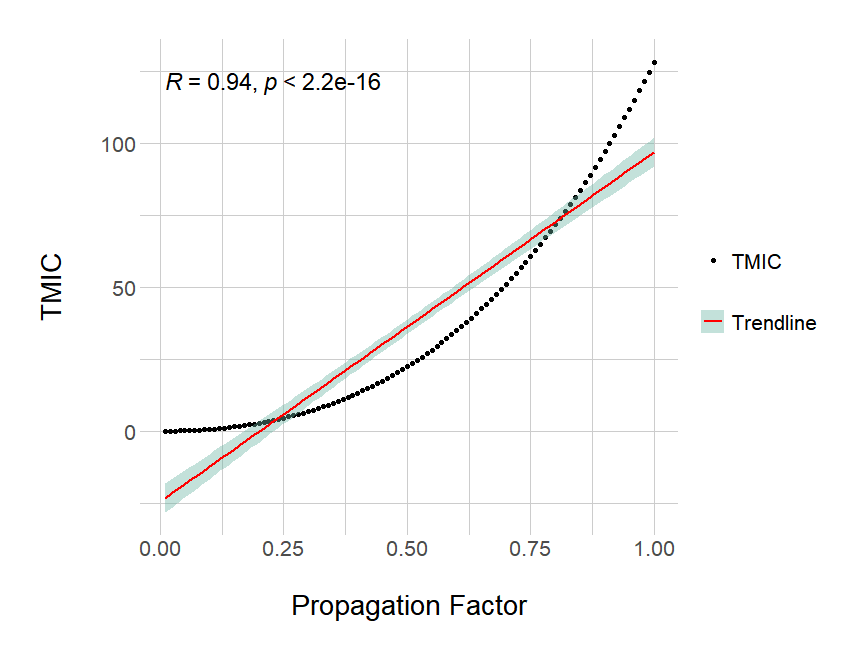
\includegraphics[width=\textwidth]{figures/results/Rplot_spoon-core_eclipse-osgi_TMIC.png}
  \end{subfigure}
  %
  \begin{subfigure}[b]{0.48\textwidth}
    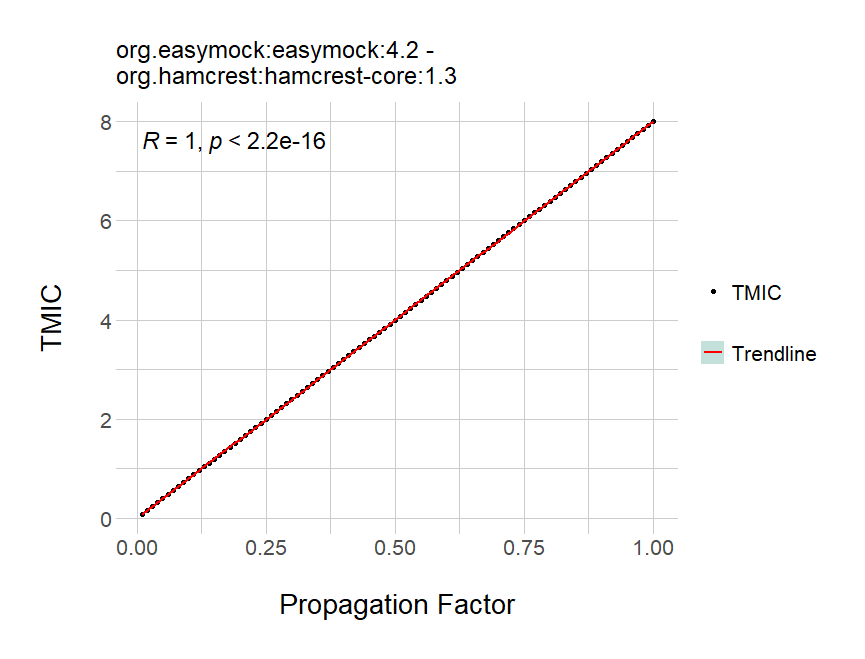
\includegraphics[width=\textwidth]{figures/results/Rplot_easymock_hamcrest_TMIC.png}
  \end{subfigure}
\caption{\texttt{TMIC} as a function of the \textit{propagation factor}, with quadratic regression (left) and linear regression (right). \textit{R} is the Pearson correlation coefficient, and \textit{p} corresponds to the confidence interval}
\label{fig:correlation-tmic}
\end{center}
\end{figure}

\begin{figure}[ht!]
\begin{center}
  \begin{subfigure}[b]{0.48\textwidth}
    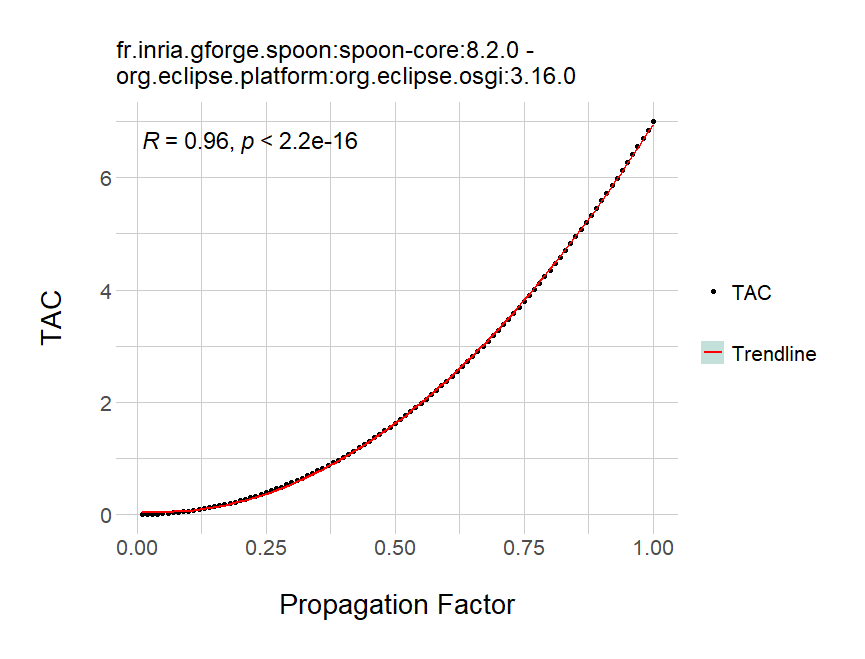
\includegraphics[width=\textwidth]{figures/results/Rplot_spoon-core_eclipse-osgi_TAC.png}
  \end{subfigure}
  %
  \begin{subfigure}[b]{0.48\textwidth}
    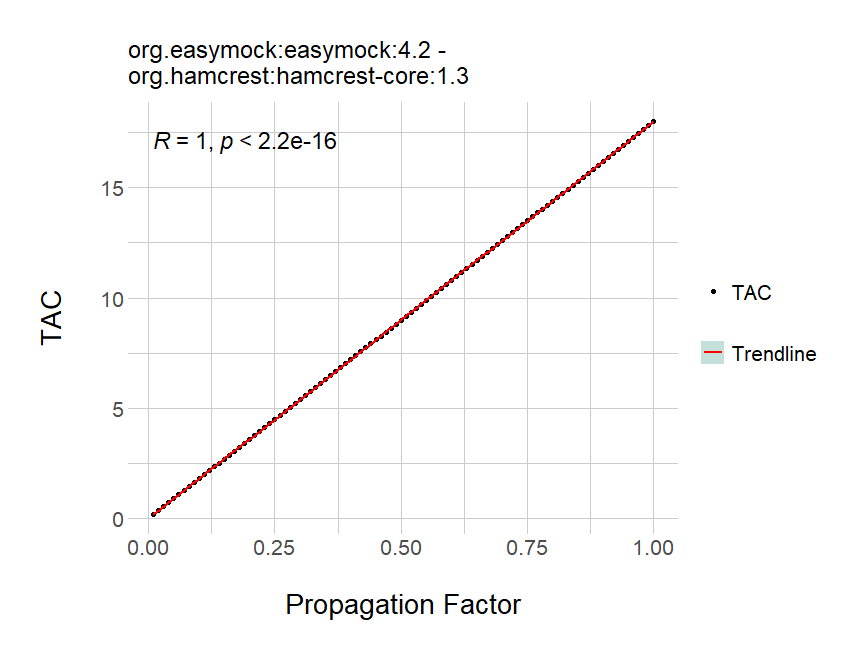
\includegraphics[width=\textwidth]{figures/results/Rplot_easymock_hamcrest_TAC.png}
  \end{subfigure}
\caption{\texttt{TAC} as a function of the \textit{propagation factor}, with quadratic regression (left) and linear regression (right). \textit{R} is the Pearson correlation coefficient, and \textit{p} corresponds to the confidence interval}
\label{fig:correlation-tac}
\end{center}
\end{figure}

\subsection{Discussion}
The sensitivity analysis results indicate a high sensitivity of the two coupling metrics to the propagation factor since there is a high correlation between these two values, the \textit{Pearson correlation coefficient} is always higher than $0.94$ (see Table \ref{table:covariance-sensitivity}).

\begin{finding}
	The value of the metrics \texttt{TMIC} and \texttt{TAC} is highly sensitive to the value of the \textit{propagation factor}.
	\label{find:high-sensitivity}
\end{finding}

In Table \ref{table:covariance-sensitivity}, we can see that the values of the covariance for \texttt{TMIC} are generally greater than those of \texttt{TAC}. This seems to be related to the fact that the values measured for \texttt{TMIC} are greater than those measured for \texttt{TAC}. Also, the cases in which the covariance is greater than $30$ seem to have greater coupling values at each distance. If we look at equation \ref{eqn:tmic}, the coupling measured at each distance ($\verb|TMICD|(L_c,L_s, \verb|distance|)$), is the value multiplied by the \textit{propagation factor}. Therefore if the \textit{propagation factor} is increased, the total value of the metric will increase more in consequence if the value of $\verb|TMICD|(L_c,L_s, \verb|distance|)$ is greater. To confirm this intuition, we create a plot to compare the covariance with the sum of the coupling measured at each distance. These plots can be seen in Figure \ref{fig:cov-value-tmic} and \ref{fig:cov-value-tac}, for \texttt{TMIC} and \texttt{TAC} respectively.

\begin{figure}[ht!]
\begin{center}
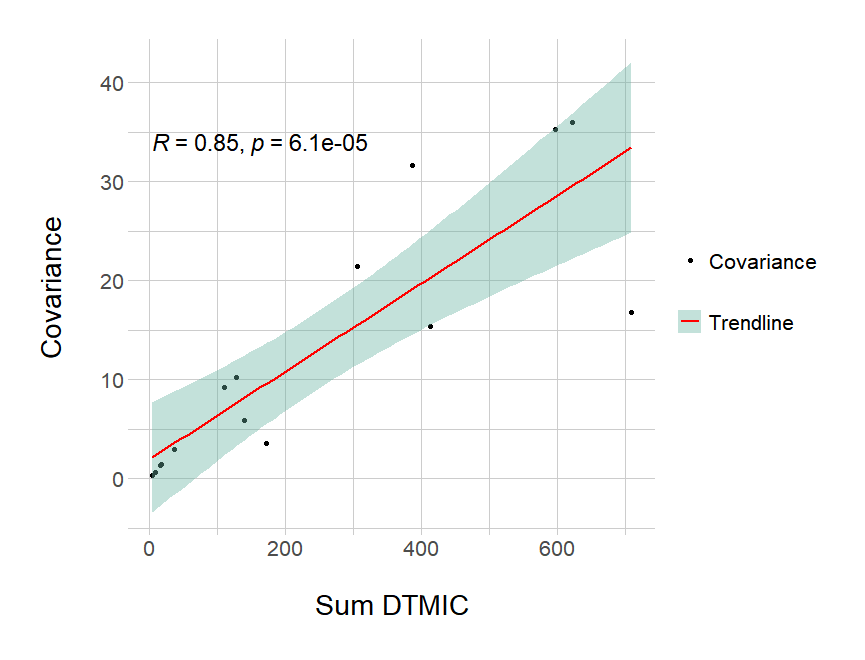
\includegraphics[width=0.7\textwidth]{figures/results/covariance-values-tmic.png}
\caption{Covariance of \textit{propagation factor} and \texttt{TMIC} as a function of the sumation of the coupling measured at each distance (\texttt{DTMIC}). \textit{p} corresponds to the confidence interval}
\label{fig:cov-value-tmic}
\end{center}
\end{figure}

\begin{figure}[ht!]
\begin{center}
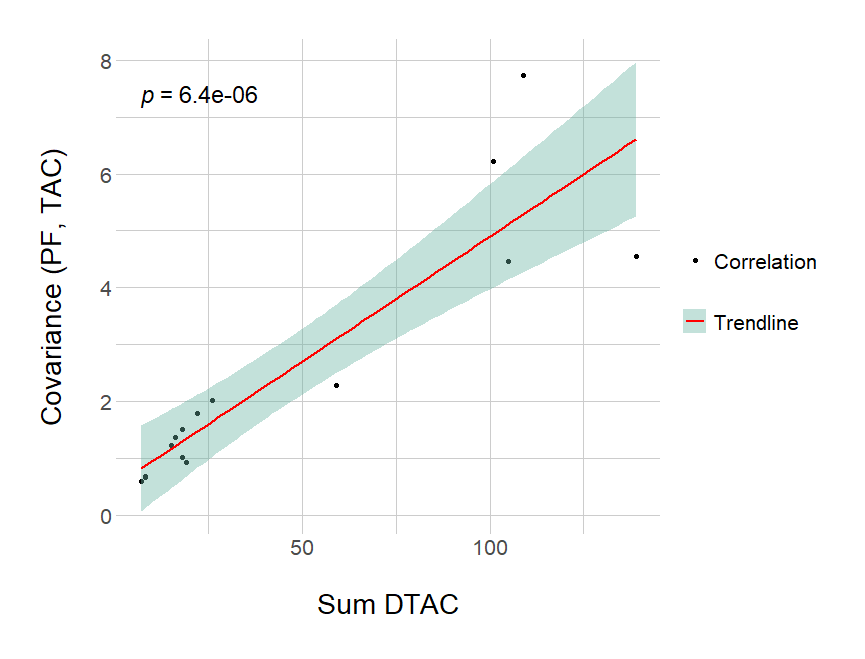
\includegraphics[width=0.7\textwidth]{figures/results/covariance-values-tac.png}
\caption{Covariance of \textit{propagation factor} and \texttt{TAC} as a function of the sumation of the coupling measured at each distance (\texttt{DTAC}). \textit{p} corresponds to the confidence interval}
\label{fig:cov-value-tac}
\end{center}
\end{figure}

Finally, in the results of the correlation coefficient between the propagation factor and the metrics, we also observe that the cases with the lowest correlation coefficients tend to be dependencies in which there is more distance between the client library and the server library. To compare the correlation and the distances, we create a plot with the correlation coefficient calculated for the sensitivity analysis and the maximum distance at which coupling is found, the plots for \texttt{TMIC} and \texttt{TAC} can be found in Figures \ref{fig:cor-dist-tmic} and \ref{fig:cor-dist-tac} respectively.

\begin{figure}[ht!]
\begin{center}
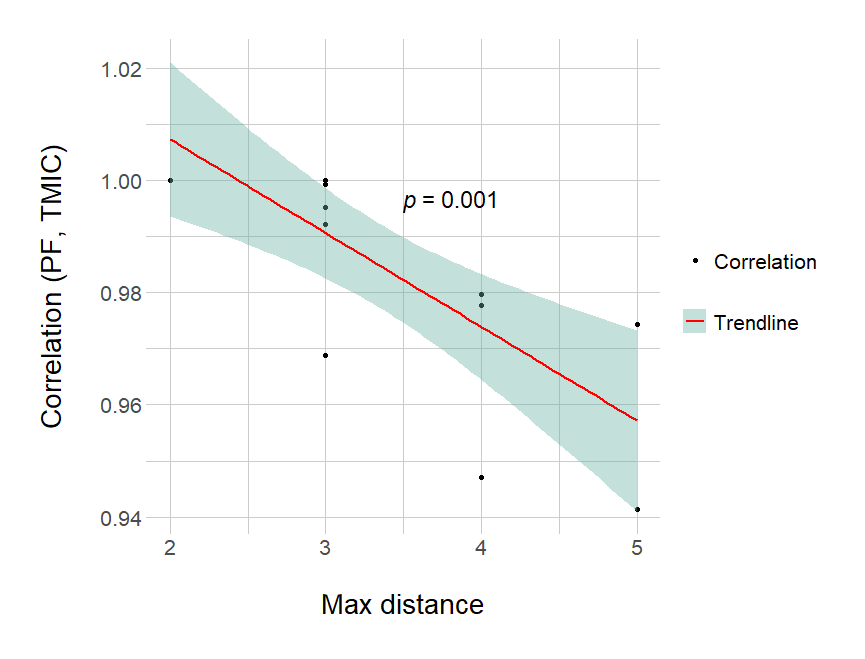
\includegraphics[width=0.7\textwidth]{figures/results/correlation_max_distance_TMIC.png}
\caption{The correlation between \textit{propagation factor} and \texttt{TMIC} as a function of the maximum distance at which coupling is measured. \textit{p} corresponds to the confidence interval}
\label{fig:cor-dist-tmic}
\end{center}
\end{figure}

\begin{figure}[ht!]
\begin{center}
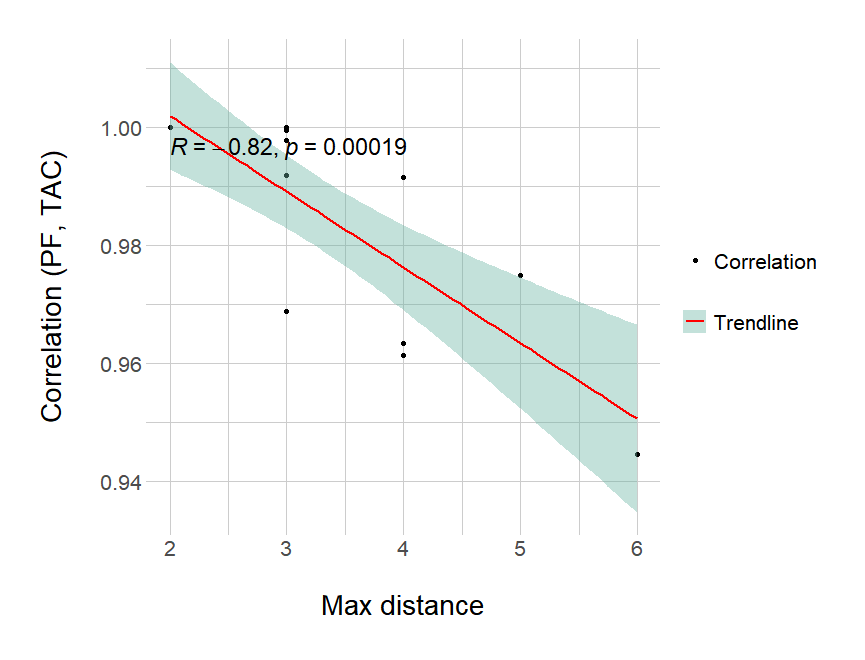
\includegraphics[width=0.7\textwidth]{figures/results/correlation_max_distance_TAC.png}
\caption{The correlation between \textit{propagation factor} and \texttt{TAC} as a function of the maximum distance at which coupling is measured. \textit{p} corresponds to the confidence interval}
\label{fig:cor-dist-tac}
\end{center}
\end{figure}

\section{Experiment 4: Expert Interviews}
This last experiment has various goals. The main one is to validate the design of the visualization. According to Munzner \cite{Munzner2009}, there are four levels at which this validation can be done:

\begin{enumerate}
  \item Domain Problem and Data Characterization
  \item Operation and Data Type Abstraction
  \item Visual Encoding and Interaction Design
  \item Algorithm Design
\end{enumerate}

In this case, we focus on the third option: Visual Encoding and Interaction Design. To carry out this validation, we designed an \textit{Expert Review} by the means of interviews. In addition, the second goal of this experiment is to evaluate the clarity and actionability of the metrics included in the model. Therefore, we added questions about clarity and actionablity, so the participants could give their view. Therefore, these two aspects of the metrics, which are included in the set of validation criteria defined by Meneely et al. \cite{Meneely2012}, can also be validated.

\subsection{Experimental set up}
The interview consists on 19 questions and a demonstration of the PoC, with two proposed scenarios in which the interviewee uses the tool. The questions are divided in four sections, which together with the demonstration divide the interview in a total of five parts:

\begin{enumerate}
  \item \textbf{Demographics:} The questions of this section are related to the interviewee's professional experience and current job.
  \item \textbf{Dependency Management:} In this part, the questions are focused on the interviewee's experience with dependency management and the tools used for this purpose.
  \item \textbf{Demonstration:} The third part is the demonstration of the tool, in which two scenarios are presented to the interviewee. During the scenarios discussion, the interviewee controls the mouse, so the person can interact directly with the tool.
  \item \textbf{Visualizations:} The section after the demonstration contains questions about the tool itself and the designed visualizations.
  \item \textbf{Metrics:} The last section focuses on the designed metrics, the clarity and comprehensibility of these, as well as actionability.
\end{enumerate}

The interviews contain three types of questions: open answer, binary, and scaled from 1 to 5. During every question, even the binary and scaled questions, the interviewee can make comments or discuss the answer. The list of questions contained in the interview, can be found in Table \ref{table:interview-questions}.

\begin{table}[p]
    \begin{center}
    \begin{tabularx}{\textwidth}{|X|l|l|}
    \hline
    Question & Section & Type \\\hline
    \hline
    1.  What is your software development role?  & Demographics & Open answer \\\hline
    2.	How many years of experience do you have as a software developer? & Demographics & Open answer \\\hline
    3.	Which programming language(s) do you usually use in your job? & Demographics & Open answer \\\hline
    4.	Which type of projects do you usually work on? & Demographics & Open answer \\\hline
    \hline
    5.	Do you have experience with dependency management? & Dependency Management & Binary \\\hline
    6.	To what extent is it important to you (or do you try) to have the dependencies up to date? & Dependency Management & Scaled \\\hline
    7.	To what extent is it important to you to monitor the vulnerabilities that your dependencies may be exploiting? & Dependency Management & Scaled \\\hline
    8.	Which tools (if any) do you use for dependency management? & Dependency Management & Open answer \\\hline
    9.	To what extent do you think the tools you used so far are helping you to maintain your dependencies? & Dependency Management & Scaled \\\hline
    \hline
    Scenario 1: You are a new maintainer of the library \textit{org.apache.flink:flink-core}. Since you have not worked in this library's development, you want to see how the dependency tree looks like. What would you look for? & Demonstration & Scenario \\\hline
    Scenario 2: You realize that a library called \textit{kryo} has a new version, which has been announced to contain breaking changes. How likely it would affect your library, and which classes are affected. & Demonstration & Scenario \\\hline
    \hline
    10.	How much do you agree that the tool is useful in the presented scenarios? & Visualizations & Scaled \\\hline
    11.	How much do you agree that managing dependencies would be easier with the presented tool? & Visualizations & Scaled \\\hline
    12.	With your job in mind, which (if any) are the most useful of the visualizations? & Visualizations & Open answer \\\hline
    13.	How much do you agree that the presented tool would be useful in your job? & Visualizations & Scaled \\\hline
    14.	Is there some other visualization or change you would like to see? For which cases do you think it would be useful? & Visualizations & Scaled \\\hline
    \hline
    15.	To what extent do you agree that the metrics are clear and comprehensible? (Answer per metric) & Metrics & Scaled \\\hline
    16.	To what extent do you agree that the metrics are useful in the described scenarios & Metrics & Scaled \\\hline
    17.	To what extent do you agree that the metrics are actionable in the sense that they give you the information you need to make a decision? & Metrics & Scaled \\\hline
    18.	Which (if any) do you think are the most useful of the metrics? Based on the tasks that you usually do in your job. & Metrics & Open answer \\\hline
    19.	Is there some other metric or change that you would like to be added to the model? In which scenarios do you think it could be useful? & Metrics & Open answer \\\hline
    \end{tabularx}
    \end{center}
    \caption{Questions of the interview}
    \label{table:interview-questions}
\end{table}

The interviews were done via \textit{Zoom}\footnote{\url{https://zoom.us/}}. \textit{Zoom} offers the possibility of sharing the control of the mouse with other participants and the option of recording the interview. The interviews are recorded to rewatch it afterward and take notes of the interviewees' answers. Therefore, the interview itself feels more like a normal conversation, and there are no pauses. The control of the mouse was shared with the interviewees to try to use the tool themselves, to get a better idea of how it works and how they would use it.

\subsection{Results}
In this section, we show the answers obtained during the interviews. The results will be discussed in section \ref{sec:discussion-interviews}: the suitability of the visualizations, as well as the clarity and actionability of the metrics.

\subsubsection{Demographics}

The roles of the 15 participants in the interviews include: Software developer, Software engineer, Technology lead, Head of innovation, Head of development, and Head of product. In some of the results, we differentiate between the answers given by developers and non-developers. In the developers' group, we consider the interviewees who answered with the role of software developer and engineer, and the rest of the interviewees are considered non-developers. The key difference is that the non-developers have tasks related to architecture or management, and therefore their needs and their perspective is different.

The years of experience range from 1 to 20, with an average of 7.13. Half of the interviewees have worked in backend development and web services systems. In addition, some of the other types of projects include mobile applications and frontend development. The languages in which the interviewees have experience can be seen in Figure \ref{fig:interview-3}.

\begin{figure}[ht!]
\begin{center}
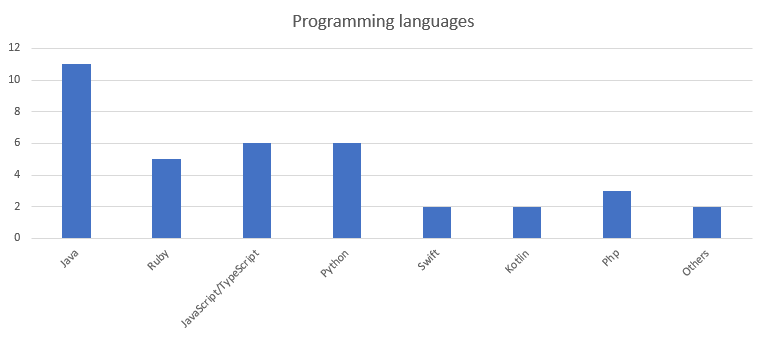
\includegraphics[width=\textwidth]{figures/interview/Question3.png}
\caption{Answers to Question 3 of the interview}
\label{fig:interview-3}
\end{center}
\end{figure}

\subsubsection{Dependency Management}

The 15 interviewees have experience with dependency management. However, some of them indicated that it is not a task that they usually perform in their jobs, but rather in personal projects or time. Figure \ref{fig:interview-6} shows the answers to question 6, regarding the importance of updating the dependencies. The reasons given by the interviewees answering \textit{Neutral} and \textit{Important} for not giving it more importance include: prioritizing the fact that the versions used are compatible, that there are no version incompatibilities with the current version used, and that the version used is stable.

\begin{figure}[ht!]
\begin{center}
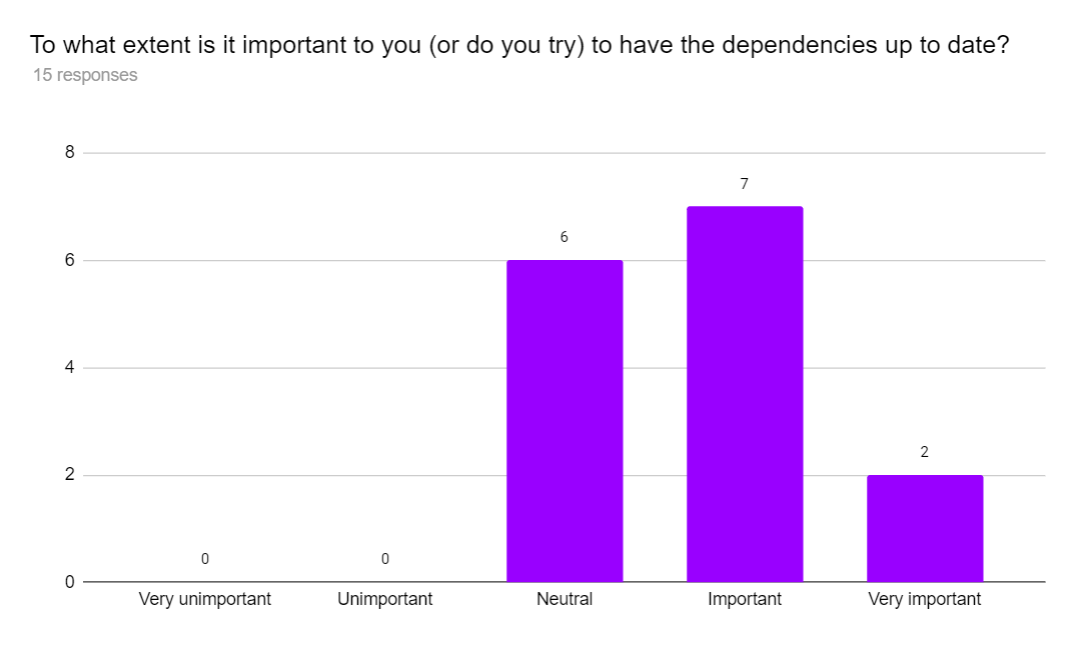
\includegraphics[width=\textwidth]{figures/interview/Question6.png}
\caption{Answers to Question 6 of the interview}
\label{fig:interview-6}
\end{center}
\end{figure}

 Figure \ref{fig:interview-7} shows the answers to question 7 about the importance of monitoring the dependencies' vulnerabilities. The interviewees which considered that the importance of monitoring the dependencies' vulnerabilities was less than \textit{Very important} reasoned about it. For example, some said that it is something that they do, but not regularly. They just update when there is a new version, to make sure that if a vulnerability has been discovered, the patch is always used. Finally, the last reason depends on the type of dependency that it is, since if it is not a customer-facing dependency, it is not that important.

\begin{figure}[ht!]
\begin{center}
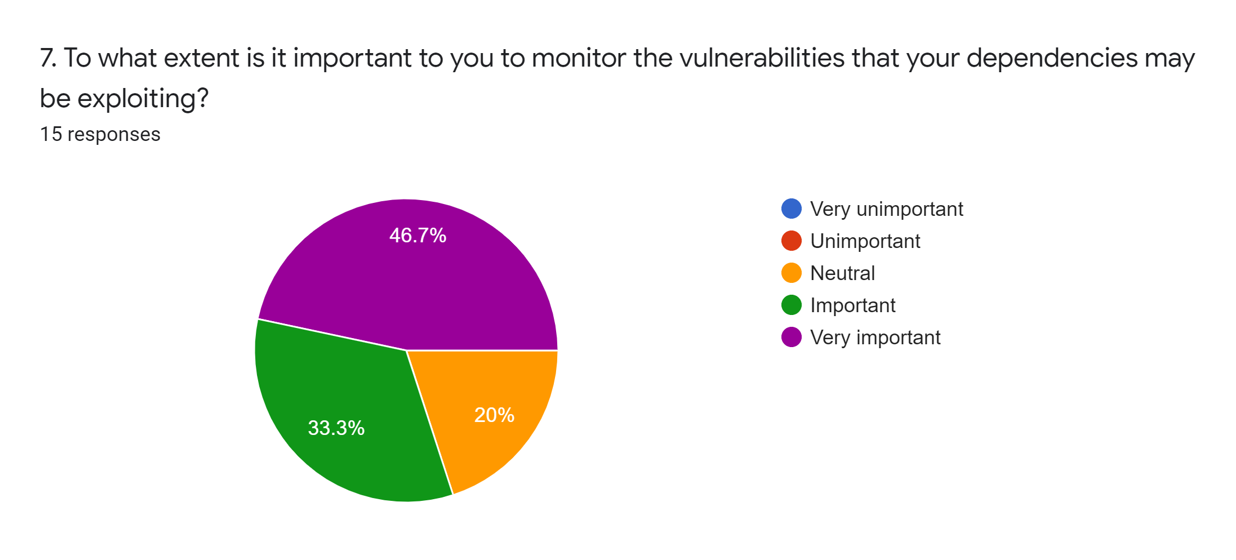
\includegraphics[width=\textwidth]{figures/interview/Question7.png}
\caption{Answers to Question 7 of the interview}
\label{fig:interview-7}
\end{center}
\end{figure}

In Figure \ref{fig:interview-8}, there are the answers to question 8. The interviewees gave more than one answer to the question, but always at least one explicitly included in the figure.

\begin{figure}[ht!]
\begin{center}
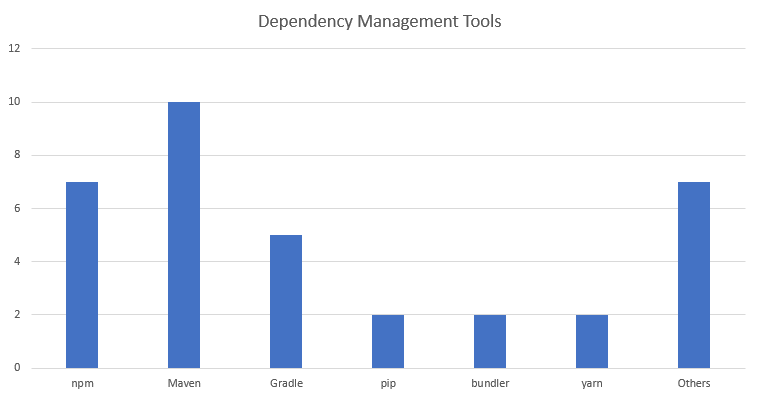
\includegraphics[width=\textwidth]{figures/interview/Question8.png}
\caption{Answers to Question 8 of the interview}
\label{fig:interview-8}
\end{center}
\end{figure}

Finally, the answers to question 9, regarding the how helpul are the tools that the interviewees use for dependency management are. The interviewees that considered the tools to be really helpful (5), compared it to not using any tool. Whilts the interviewees giving lower marks (2-3), considered that features are missing. Mainly, they considered that the basic needs are covered, however some more detailed information about how to manage the dependencies is not there.

\begin{figure}[ht!]
\begin{center}
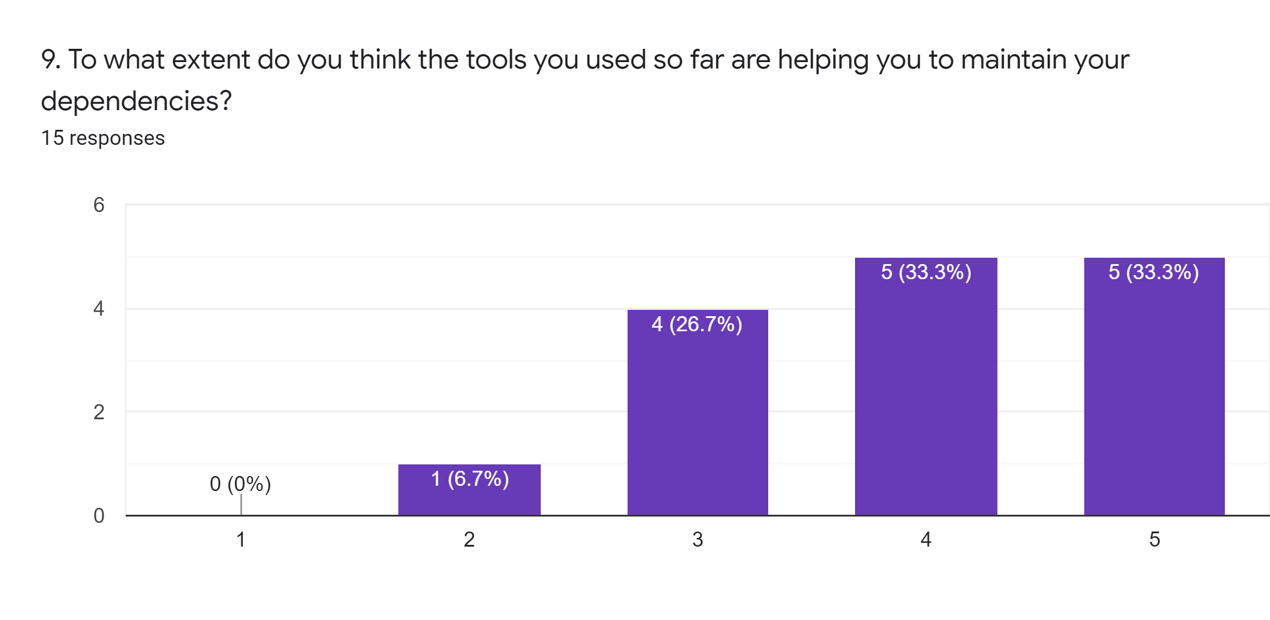
\includegraphics[width=\textwidth]{figures/interview/Question9.png}
\caption{Answers to Question 9 of the interview}
\label{fig:interview-9}
\end{center}
\end{figure}

\subsubsection{Visualizations}

The answers of the interviewees to question 10 about the tool's usefulness are displayed in Figure \ref{fig:interview-10}. Some of the interviewees' reasons for not giving it the maximum grade are the need for improvement in some aspects of both the visualization and the metrics and being useful for some very specific scenarios.

\begin{figure}[ht!]
\begin{center}
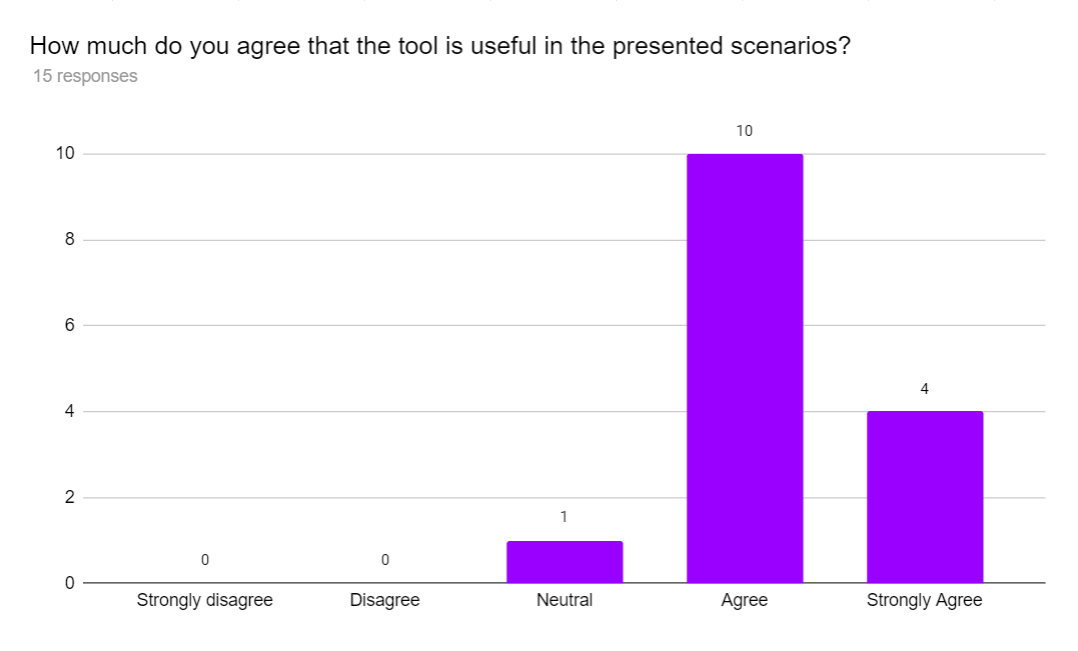
\includegraphics[width=\textwidth]{figures/interview/Question10.png}
\caption{Answers to Question 10 of the interview}
\label{fig:interview-10}
\end{center}
\end{figure}

Figure \ref{fig:interview-11} we can see the results for Question 11. In this case, the interviewees who answered \textit{Disagree} or \textit{Neutral} considered that the tool is meant for some very specific cases, which are not very likely to be needed. The other interviewees agreed that the tool would probably not be used daily, but would make some tasks easier, such as those discussed in the scenarios.

\begin{figure}[ht!]
\begin{center}
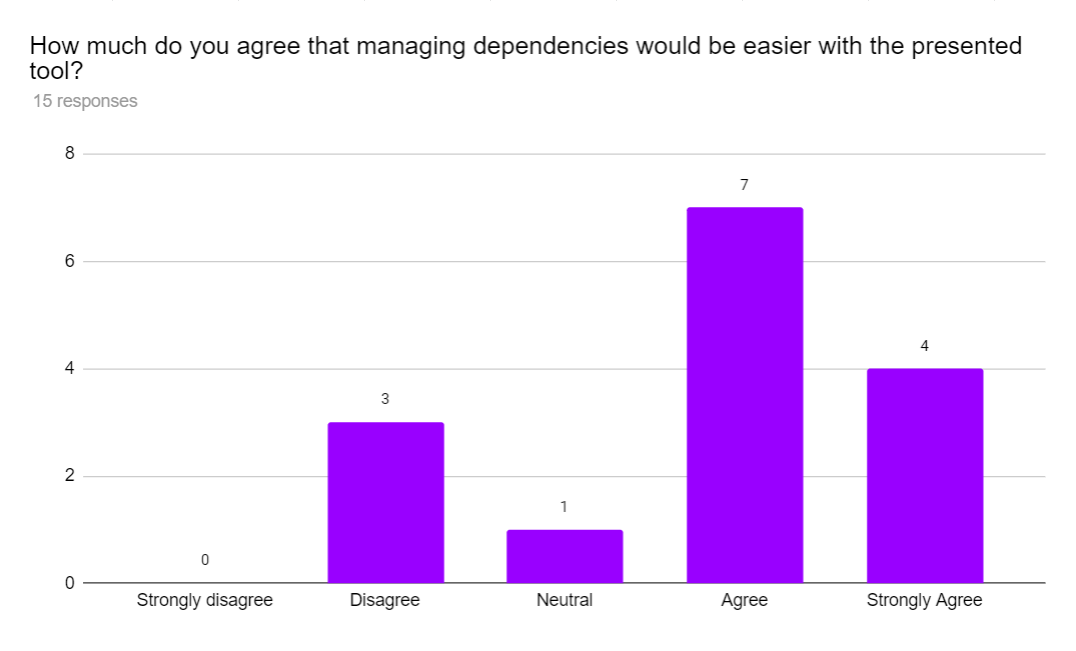
\includegraphics[width=\textwidth]{figures/interview/Question11.png}
\caption{Answers to Question 11 of the interview}
\label{fig:interview-11}
\end{center}
\end{figure}

For Question 12, about which visualizations are most useful, most of the interviews answered with more than one visualization. Table \ref{table:interview-12} summarizes the answers.

\begin{table}[ht!]
    \begin{center}
    \begin{tabular}{|c|c|c|}
    \hline
    Tree      & Table     & Barchart \\
    \hline\hline
    $\odot$   & $\oplus$  & ~        \\\hline
    ~	        & ~	        & $\oplus$ \\\hline
    $\oplus$  & ~         & $\oplus$ \\\hline
    $\oplus$	& ~         & ~        \\\hline
    $\oplus$	& $\odot$	  & $\oplus$ \\\hline
    $\oplus$	& ~         & $\odot$  \\\hline
    $\odot$	  & $\oplus$	& ~        \\\hline
    $\oplus$	& $\oplus$	& $\oplus$ \\\hline
    ~	        & ~	        & $\oplus$ \\\hline
    $\odot$	  & $\odot$	  & $\oplus$ \\\hline
    $\oplus$	& $\oplus$	& $\oplus$ \\\hline
    $\oplus$	& ~	        & ~        \\\hline
    $\oplus$	& $\oplus$	& $\oplus$ \\\hline
    $\odot$	  & ~	        & $\oplus$ \\\hline
    $\oplus$	& $\oplus$	& $\oplus$ \\\hline
    \end{tabular}
    \end{center}
    \caption{Answers to Question 12 of the interview. $\oplus$ indicates that the interviewee considered that visualization to be the most useful, the $\odot$ is used when the visualization was considered useful but in a clear second position, and an empty cell means that the the visualization was not mentioned.}
    \label{table:interview-12}
\end{table}

The answers to Question 13 are shown in Figure \ref{fig:interview-13}. Just as in Question 11, the reason given by the interviewees who answered \textit{Disagree} or \textit{Neutral} are that the tasks for which the tool is useful are not one of the regular tasks in their job.

\begin{figure}[ht!]
\begin{center}
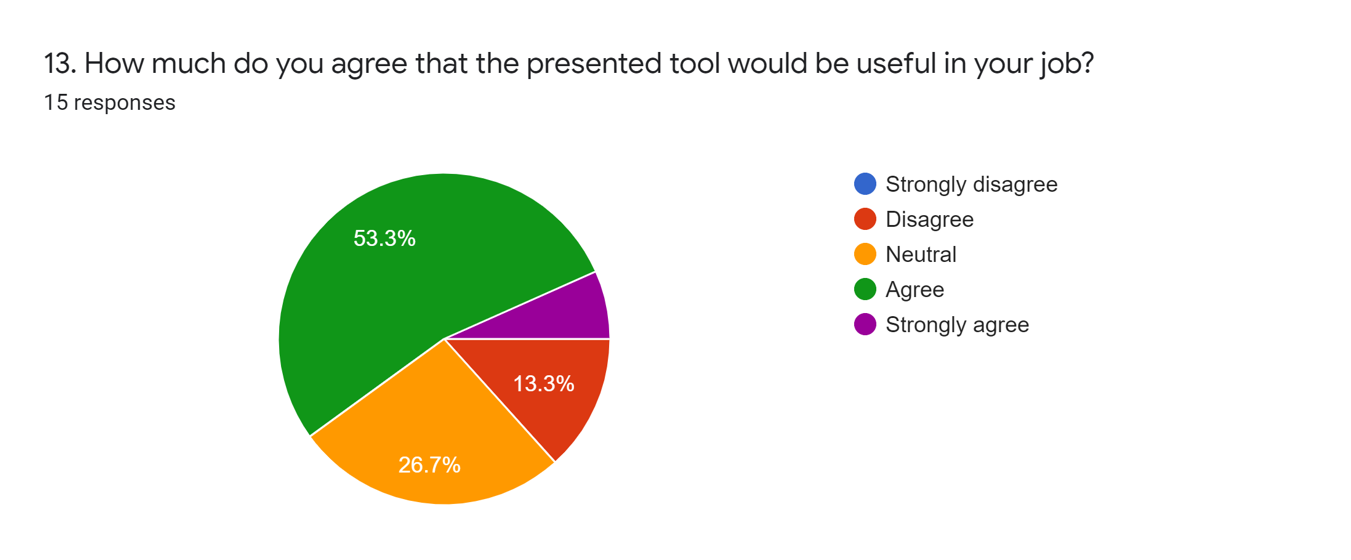
\includegraphics[width=\textwidth]{figures/interview/Question13.png}
\caption{Answers to Question 13 of the interview}
\label{fig:interview-13}
\end{center}
\end{figure}

With Question 14, the interviewees gave their suggestions for improvements to the current visualizations and completely new visualizations. The list of suggestions can be found below:

\begin{itemize}
  \item Add tree visualization at the class level.
  \item List with the classes and methods used from a library.
  \item Add a decision-making model, indicating which actions should be taken.
  \item Visualization to know how much of the system is depending on a library.
  \item Smart visualization displaying some potential problems: the freshness of the dependency, multiple versions of the same library being used.
  \item Color legend in the tree graph.
  \item Tooltip with a description of the metrics of the model.
  \item Display the licenses of the dependencies.
  \item Change the bar chart for a table.
  \item Possibility to move and reorganize the nodes of the tree.
  \item Turn the features into a command interface to be unattended running in the build pipeline.
\end{itemize}

\subsubsection{Metrics}

The answers to question 15 can be found in Figure \ref{fig:interview-15}; for each metric, the number of times an interviewee answered with each number of the options. In addition, Table \ref{table:interview-15} shows the average mark given to each metric, first considering only the marks given by developers, then by non-developers, and finally, the total average.

\begin{figure}[ht!]
\begin{center}
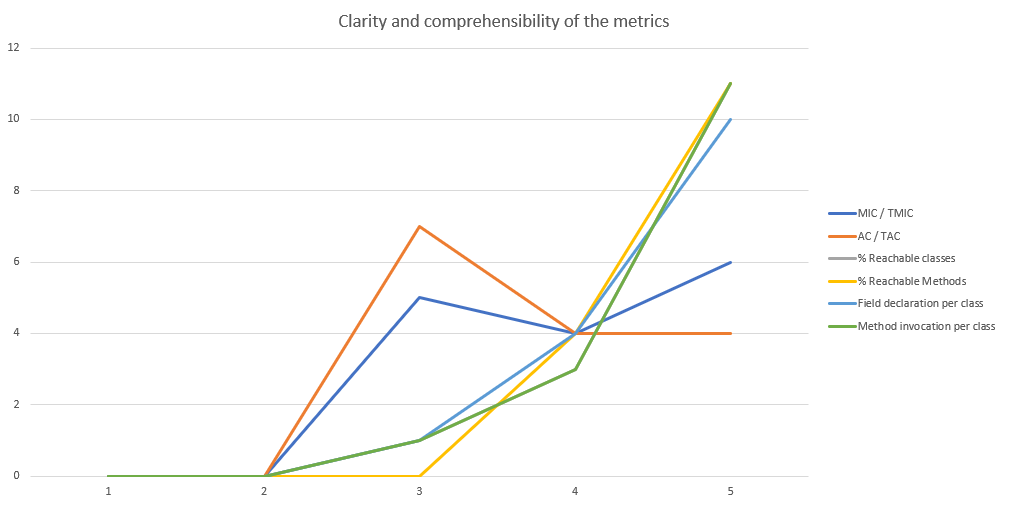
\includegraphics[width=\textwidth]{figures/interview/Question15.png}
\caption{Answers to Question 15 of the interview}
\label{fig:interview-15}
\end{center}
\end{figure}

\begin{table}[ht!]
    \begin{center}
    \begin{tabular}{|l|l|l|l|}
    \hline
    Metric                      & Average developers  & Average non-developers  & Total Average \\
    \hline
    MIC/TMIC                    & 3.8                 & 4.6               & 4.06 \\
    AC/TAC                      & 3.6                 & 4.2               & 3.8 \\
    \% Reachable classes        & 4.6                 & 4.8               & 4.66 \\
    \% Reachable methods        & 4.8                 & 4.6               & 4.73 \\
    Field declaration per class & 4.8                 & 4.2               & 4.6 \\
    Method invocation per class & 4.8                 & 4.4               & 4.66 \\
    \hline
    \end{tabular}
    \end{center}
    \caption{Results Question 15: Average marks of the metrics, given by developers, non-developers, and all}
    \label{table:interview-15}
\end{table}

In Figure \ref{fig:interview-16}, there are the answers to question 16 of the interview. The reasons for not giving the metrics the best grade include that it would be more useful if the metrics suggested as missing in question 19 were included. It was also suggested that context is missing for some metrics (e.g., the absolute number of reachable methods and classes, risk assessment for the coupling metrics).

\begin{figure}[ht!]
\begin{center}
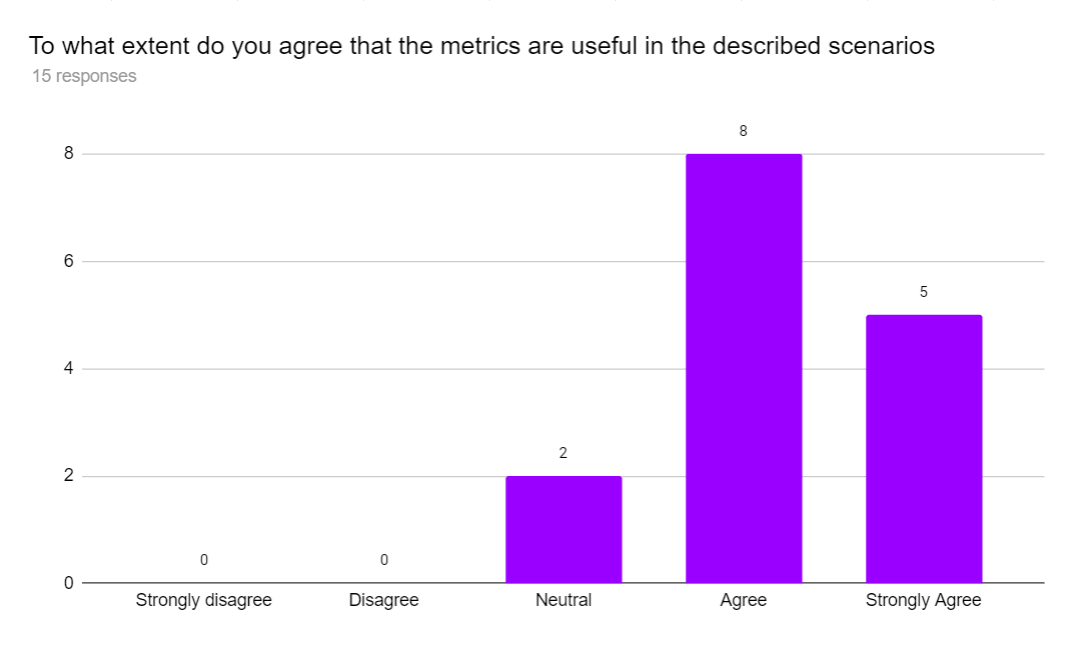
\includegraphics[width=\textwidth]{figures/interview/Question16.png}
\caption{Answers to Question 16 of the interview}
\label{fig:interview-16}
\end{center}
\end{figure}

The answers to question 17 can be found in Figure \ref{fig:interview-17}. The interviewees who gave the grade \textit{Neutral} reasoned that the metrics need some improvements to be trully actionable and that there is information that still can only be found in other places. The interviewees who answered \textit{Agree} suggested that the model's metrics are a good starting point to know which actions to take to start with.

\begin{figure}[ht!]
\begin{center}
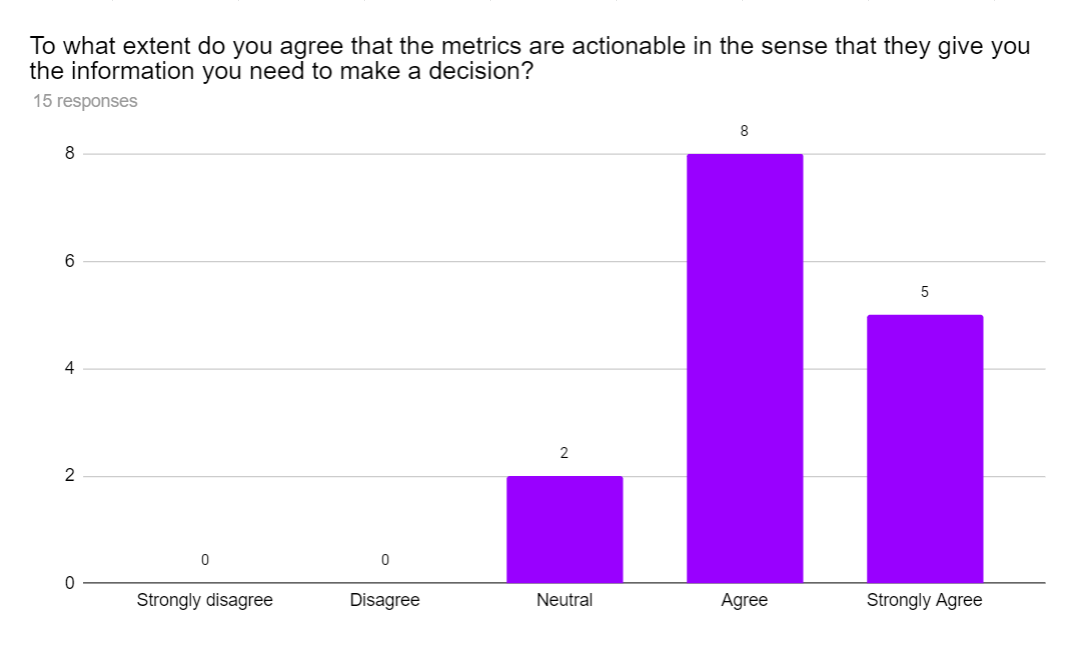
\includegraphics[width=\textwidth]{figures/interview/Question17.png}
\caption{Answers to Question 17 of the interview}
\label{fig:interview-17}
\end{center}
\end{figure}

For question 18, the interviewees answered with which metrics they considered more useful. Their answers can be found in Table \ref{table:interview-18}.

\begin{table}[ht!]
    \begin{center}
    \begin{tabular}{|c|c|c|c|c|c|l|}
    \hline
    \rot{MIC / TMIC}	& \rot{AC / TAC}	& \rot{\% Reachable classes}	& \rot{\% Reachable Methods}	& \rot{Field declaration per class}	& \rot{Method invocation per class    } & \rot{Role} \\
    \hline\hline
    $\oplus$  & ~	       & $\oplus$	& ~	        & ~	        & ~        & Developer \\\hline
    ~	        & ~	       & $\oplus$	& $\oplus$	& ~	        & ~        & Developer \\\hline
    ~	        & ~	       & $\oplus$	& $\oplus$  & ~	        & ~        & Developer \\\hline
    ~	        & ~	       & ~	      & ~	        & $\odot$	  & $\oplus$ & Developer \\\hline
    ~	        & ~	       & $\oplus$	& $\oplus$	& ~	        & ~        & Developer \\\hline
    ~	        & ~	       & $\oplus$	& $\oplus$	& ~	        & ~        & Developer \\\hline
    $\oplus$	& ~	       & $\oplus$	& $\oplus$	& ~	        & ~        & Non-developer   \\\hline
    $\oplus$	& ~	       & ~	      & ~	        & ~	        & ~        & Non-developer   \\\hline
    $\oplus$	& $\oplus$ & $\oplus$	& $\oplus$	& ~	        & ~        & Developer \\\hline
    ~	        & ~	       & $\oplus$	& $\oplus$	& $\oplus$	& $\oplus$ & Developer \\\hline
    $\oplus$	& $\oplus$ & $\oplus$	& $\oplus$	& $\oplus$  & $\oplus$ & Non-developer   \\\hline
    $\oplus$	& $\oplus$ & ~	      & ~	        & ~	        & ~        & Developer \\\hline
    $\oplus$	& $\oplus$ & ~	      & ~	        & ~	        & ~        & Non-developer   \\\hline
    ~	        & ~        & $\oplus$ & $\oplus$	& ~         & ~        & Developer \\\hline
    $\oplus$	& ~	       & $\oplus$ & ~	        & ~	        & ~        & Non-developer   \\\hline
    \end{tabular}
    \end{center}
    \caption{Answers to Question 18 of the interview. $\oplus$ indicates that the interviewee considered the metric to be the most useful, the $\odot$ is used when the metric was considered useful but in a clear second position, and an empty cell means that the the metric was not mentioned.}
    \label{table:interview-18}
\end{table}

Finally, the suggestions made for improving the current metrics or adding new ones, in the answers of question 19, can be found in the list below:

\begin{itemize}
  \item Min, max, and mean of the coupling metrics.
  \item How much of the client is depending on the server library.
  \item A list of the reachable methods and classes.
  \item The absolute number of reachable methods and classes.
  \item Freshness indicator.
  \item Aggregate of the coupling metrics.
  \item Muber of files of the client using the server library.
  \item Lines of code of the client affected by the dependency.
  \item Code reuse: a combination of the metrics.
\end{itemize}

\subsection{Discussion}\label{sec:discussion-interviews}
In this section, we discuss the answers to the interviews, divided into sections. First, there is a discussion on the interviewees' general evaluation, according to their role.

We have found a difference in how the interviewees evaluate the model and the visualizations according to whether the interviewee's main focus is development or not.

The developers want more information that can be directly transformed into development actions. For example, they suggested seeing the list of reachable methods of the dependencies, which can answer a vulnerable method is used or not. Another example is the lines of code where the calls to a dependency are made, so the developer can directly go to that line of code to make the necessary changes.

However, non-developers are interested in more high-level information. One of the suggestions made was to create a metric regarding how much of the client library depends on the server library. Also, how widespread the usage is in the client library. These two metrics would be related to the architecture of the system.

Furthermore, there is also an indicator of this difference in their answers to the preferred metric. The coupling metrics are more useful at an architectural level to understand how much a client depends on a server library. In Table \ref{table:interview-18}, we see the the interviewees with non-developer role, always mentioned at least \texttt{MIC}/\texttt{TMIC} as the most useful metric. If we compare the average marks of the developers and non-developers in Table \ref{table:interview-15}, we can see this same difference. The marks given by non-developers to the coupling metrics are higher than those given by developers.

\subsubsection{Dependency Management}
With the questions answered in the \textit{Dependency Management} section, we know that all the interviewees have experience with this type of task. Also, the interviewees considered it more important to monitor the dependencies' vulnerabilities than the update to the last version (see Figures \ref{fig:interview-6}, and \ref{fig:interview-7}). This is also confirmed by some interviewees' comments, saying that the main reason to update a dependency is to avoid being affected by possible vulnerabilities.

\subsubsection{Visualizations}
When asked about the tool's usefulness, there is a general agreement that the tool is useful in the scenarios discussed during the interview, Figure \ref{fig:interview-10}. There are some negative answers to whether the tool can make dependency management easier. However, most of the comments about these answers are related to the tool being useful for particular cases. Therefore, the negative responses are not associated with the tool, not making the tasks easier.

\begin{finding}
	There is a consensus that the created tool is useful in certain scenarios related to dependency management.
	\label{find:tool-useful}
\end{finding}

In the answers to Question 12, only four interviewees answer only one of the visualizations (see Table \ref{table:interview-12}). Some of the other interviewees also commented that there is value in combining the perspectives in the visualizations. Each visualization has a point of view, which adds to the value of the entire tool. The \textit{Tree} visualization gives an understanding of the hierarchy of the dependencies and where the transitive dependencies come from. The \textit{Table} visualization makes it possible to compare the metrics, and therefore, the degree of dependence. Finally, the \textit{Barchart} gives a more detailed view of the impact of the dependencies in the client library.

\begin{finding}
	It is important to have a different perspective on a system's dependencies in the visualizations to have a complete understanding of the dependency tree.
	\label{find:different-perspectives}
\end{finding}

With the last question about the visualizations, the interviewees suggested some improvements to be made. Certain suggestions are small improvements in terms of interaction with the visualizations, and some other additions to make it easier to use. According to the research method, the next step would be implementing some of these suggestions and doing more interviews. However, due to time limitations, we cannot do these tasks.

Also, some interviewees expressed a need to integrate the different sources of information about dependency management. This data includes vulnerability data, the new versions available of the dependencies, and the licenses of the libraries used. Some related suggestions into making this tool's features into another type of tool are to make it an IDE Plugin and a command interface. Hence, there is a general interest in the tool, but it might be important to consider changing the format in which these are supplied.

\subsubsection{Metrics}
Regarding the clarity and comprehensibility of the metrics, the interviewees' average grade for all the metrics is positive, being a 3.8/5, the lowest one, and a 4.73/5 the highest one, as shown in Table \ref{table:interview-15}.

\begin{finding}
	There is a consensus that the metrics defined in this model are clear and comprehensible.
	\label{find:clear-comprehensible}
\end{finding}

The metrics with the lowest grade are the coupling metrics. As confirmed by the comments of the question about the model's actionability, most of the interviewees agreed that the coupling metrics are harder to understand since there is not a clear scale. Therefore, a number gives some information on the dependency itself and how it compares to the rest of dependencies in the tree, but there is no clear meaning that indicates if a certain value is "good" or "bad."

\begin{finding}
	The coupling metrics could be improved with a clear scale or rating evaluation.
	\label{find:coupling-scale}
\end{finding}

The answers to Question 16, about the usefulness of the model, are mainly positive (see Figure \ref{fig:interview-16}). Just as in the visualizations, the interviewees giving the lowest marks reasoned that the need to have such a detailed evaluation of the dependencies is not necessary daily.

\begin{finding}
	The model is useful for dependency management. However, it is not needed for the most common and regular tasks.
	\label{find:model-useful}
\end{finding}

With respect to question 18, regarding which are the most useful metrics in the model, the metrics that got more votes are the coverage metrics, as shown in Table \ref{table:interview-18}. This result is consistent with the answers to Question 15, in which the coverage metrics have two of the highest average scores. Also, just as in the visualizations, some interviewees commented that it is the different perspectives given by each of the metrics making the model more useful.

In the last question of the interviews, we gathered suggestions about the model's metrics and can also be grouped into changes to current metrics and new metrics. One of the main suggestions obtained is to create a combination of the coupling metrics, have a general evaluation, and dive into the detail with the current metrics. The users would then have a general indicator, which can already point them to the dependencies that need a more detailed look.

\begin{finding}
	There is an interest in a general metric indicating the general degree of dependency as a combination of the model's existing metrics.
	\label{find:general-metric}
\end{finding}

We have also obtained some suggestions, which are modifications to the current metrics. For example, having the absolute number of reachable methods or classes and the list of their names. It should be evaluated, which is the need for this information, and in which cases it would be useful.

Finally, one of the suggestions to improve the actionability of the coupling metrics is to create a risk profile of these metrics by evaluating the common values of these metrics and the outliers. This suggestion is further investigated in the following experiment.

\section{Experiment 5: Benchmarking}
One of the main remarks received for the coupling metrics during the interviews is that there is no clear scale for those metrics. Therefore, the metrics' value can be hard to interpret, since there is no indicator of which number is very high or very low.

Hence, we have benchmarked the values of the metrics \texttt{MIC}, \texttt{AC}, \texttt{TMIC}, and \texttt{TAC}. The goal is to understand, which is the distribution of the values and be able to indicate which are the outliers of these metrics.

\subsection{Experimental set up}
To execute this experiment, we have set a new request in the backend of the PoC. This request should contain the path to a \textit{.txt} file, which includes three different columns, tab-delimited. Each row represents a Maven artifact, and for each column it indicates: \textit{group id}, \textit{artifact id}, and \textit{version}.

Then, the calculation of the metrics of the model is performed. For each analyzed dependency, the value of the benchmarked metrics is stored. The result consists on 4 different \textit{.csv} files. The first two contain all the different values of the \texttt{MIC} and \texttt{AC} metrics. The last files represent the values of the transitive coupling metrics, represented in three columns. The first, the dependency id, the second the distance, and the third the value calculated at that distance. Therefore, more than one row might be used to represent the \texttt{TMIC} or \texttt{TAC} of a dependency.

\subsection{Results}

We have analyzed a total of $299$ direct dependencies and $470$ transitive dependencies, obtained from analyzing a set of Maven libraries (see list of libraries in Appendix \ref{appendix:data-set}). We filtered out zero values since it means that there is no coupling in this case, and we plot the rest of the values. In Figures \ref{fig:MIC-benchmark} and \ref{fig:AC-benchmark}, we show the histograms representing the distribution of the values of \texttt{MIC} and \texttt{AC} respectively.

\begin{figure}[ht!]
\begin{center}
  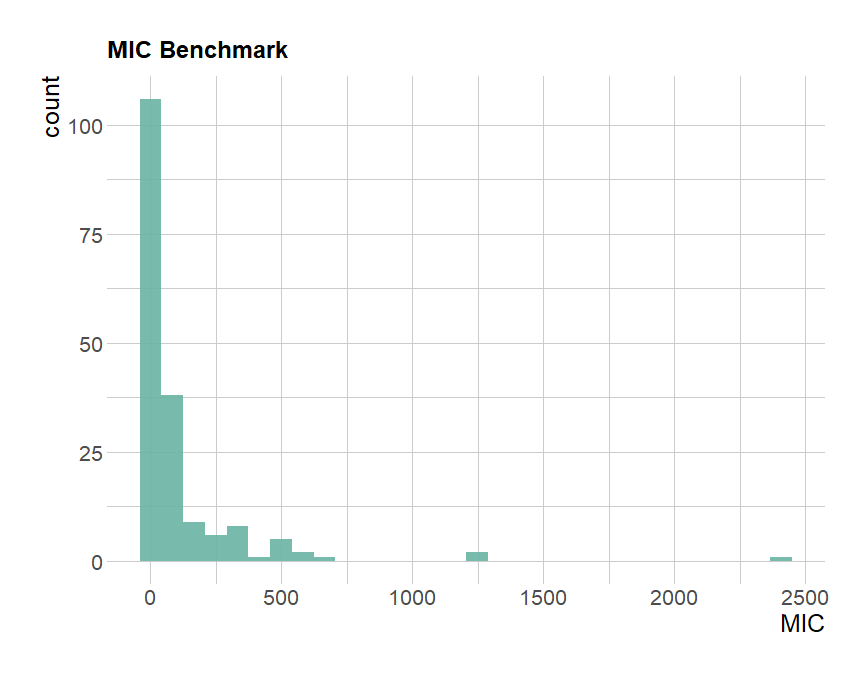
\includegraphics[width=0.7\textwidth]{figures/benchmark/MIC_benchmark.png}
  \caption{Histogram \texttt{MIC} benchmark, 60 bins}
  \label{fig:MIC-benchmark}
\end{center}
\end{figure}

\begin{figure}[ht!]
\begin{center}
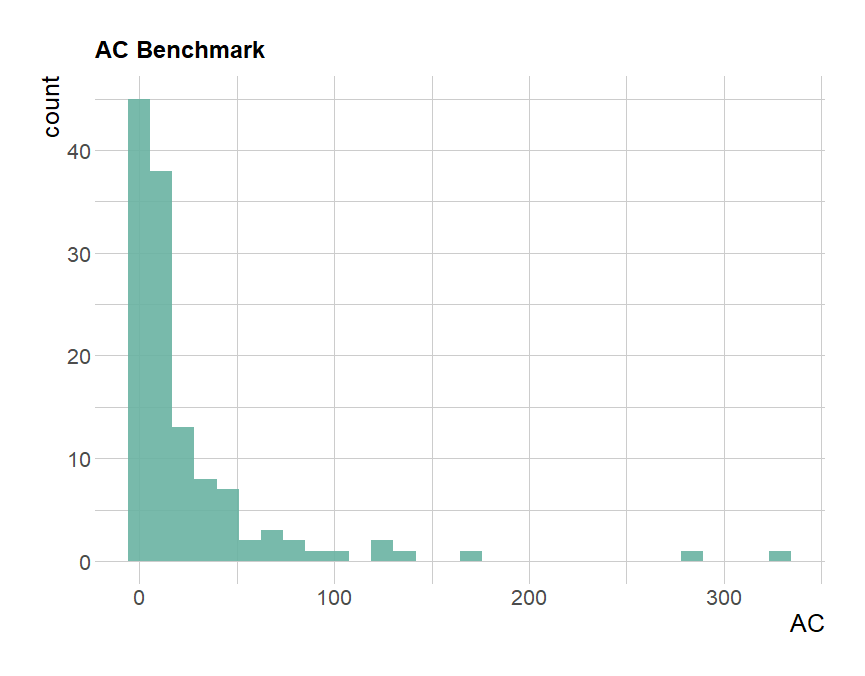
\includegraphics[width=0.7\textwidth]{figures/benchmark/AC_benchmark.png}
\caption{Histogram \texttt{AC} benchmark, 60 bins}
\label{fig:AC-benchmark}
\end{center}
\end{figure}

For the transitive metrics, namely \texttt{TMIC} and \texttt{TAC}, we have calculated the benchmarking with different values for the \textit{propagation factor}. The histogram of the benchmarks for metrics \texttt{TMIC} and \texttt{TAC} with propagation factor $1$, $0.5$, and $0.1$, can be found in Figures \ref{fig:TMIC-benchmark-1}, \ref{fig:TAC-benchmark-1}, \ref{fig:TMIC-benchmark-0.5} and \ref{fig:TAC-benchmark-0.5}, \ref{fig:TMIC-benchmark-0.1}, and \ref{fig:TAC-benchmark-0.1}, respectively.

\begin{figure}[ht!]
\begin{center}
  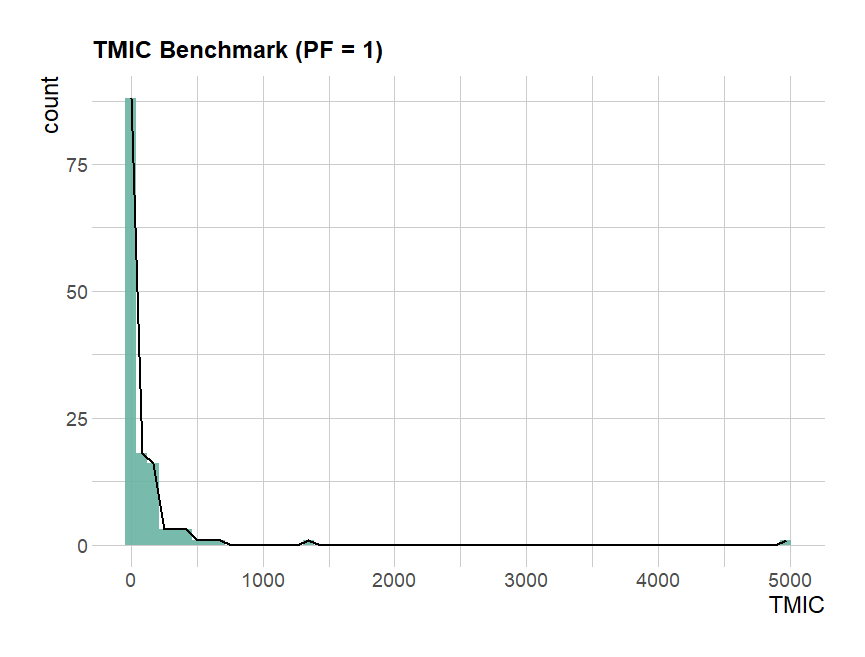
\includegraphics[width=0.7\textwidth]{figures/benchmark/TMIC_PF_1.png}
  \caption{Histogram \texttt{TMIC} benchmark, propagation factor = 1, 60 bins}
  \label{fig:TMIC-benchmark-1}
\end{center}
\end{figure}

\begin{figure}[ht!]
\begin{center}
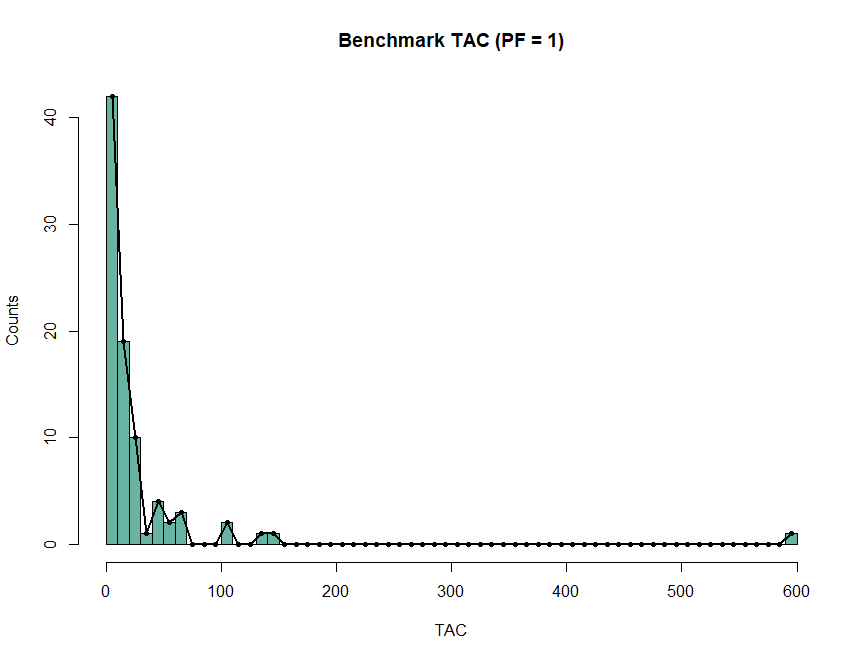
\includegraphics[width=0.7\textwidth]{figures/benchmark/TAC_PF_1.png}
\caption{Histogram \texttt{TAC} benchmark, propagation factor = 1, 60 bins}
\label{fig:TAC-benchmark-1}
\end{center}
\end{figure}

\begin{figure}[ht!]
\begin{center}
  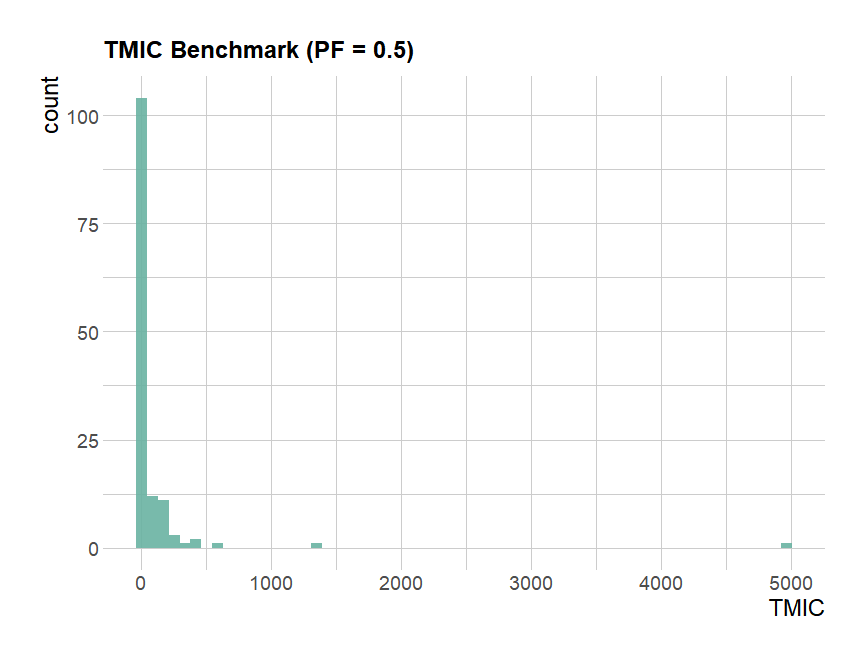
\includegraphics[width=0.7\textwidth]{figures/benchmark/TMIC_PF_0.5.png}
  \caption{Histogram \texttt{TMIC} benchmark, propagation factor = 0.5, 60 bins}
  \label{fig:TMIC-benchmark-0.5}
\end{center}
\end{figure}

\begin{figure}[ht!]
\begin{center}
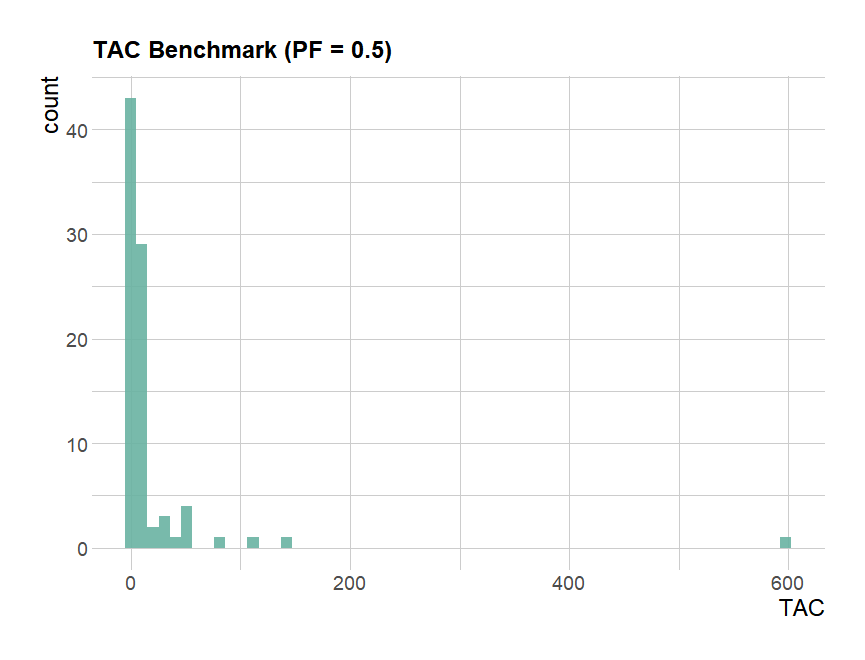
\includegraphics[width=0.7\textwidth]{figures/benchmark/TAC_PF_0.5.png}
\caption{Histogram \texttt{TAC} benchmark, propagation factor = 0.5, 60 bins}
\label{fig:TAC-benchmark-0.5}
\end{center}
\end{figure}

\begin{figure}[ht!]
\begin{center}
  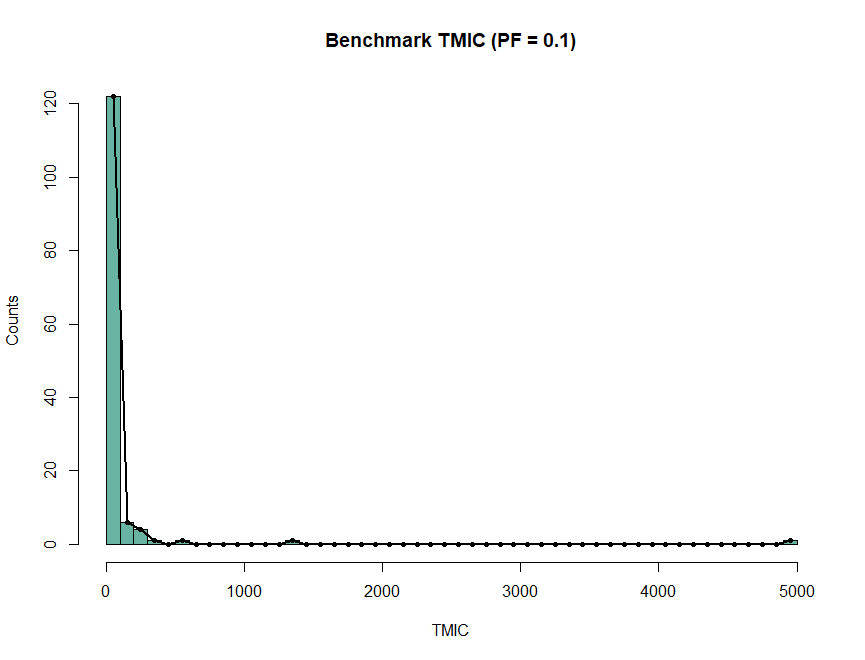
\includegraphics[width=0.7\textwidth]{figures/benchmark/TMIC_PF_0.1.png}
  \caption{Histogram \texttt{TMIC} benchmark, propagation factor = 0.1, 60 bins}
  \label{fig:TMIC-benchmark-0.1}
\end{center}
\end{figure}

\begin{figure}[ht!]
\begin{center}
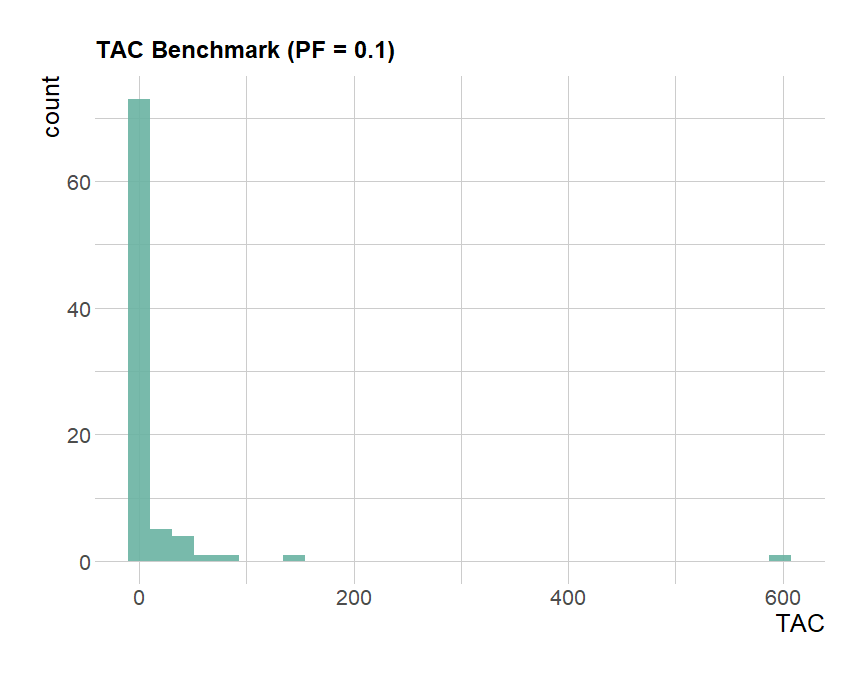
\includegraphics[width=0.7\textwidth]{figures/benchmark/TAC_PF_0.1.png}
\caption{Histogram \texttt{TAC} benchmark, propagation factor = 0.1, 60 bins}
\label{fig:TAC-benchmark-0.1}
\end{center}
\end{figure}

Finally, we also generated 70th, 80th, and 90th percentiles of each of the metrics, which can be found in Table \ref{table:percentiles}.

\begin{table}[ht!]
    \begin{center}
    \begin{tabular}{|r|l|l|l|}
    \hline
    \diagbox{\textbf{Metric}}{\textbf{Percentile}} & \textbf{70th} & \textbf{80th} & \textbf{90th} \\ \hline\hline
    \textbf{MIC} & 79.00 & 118.80 & 305.40 \\ \hline
    \textbf{AC} & 21.50 & 35.00 & 61.00 \\ \hline
    \textbf{TMIC (PF = 1)} & 59.50 & 129.00 & 215.00 \\ \hline
    \textbf{TAC (PF = 1)} & 19.50 & 24.00 & 56.00 \\ \hline
    \textbf{TMIC (PF = 0.5)} & 30.37 & 87.00 & 141.87 \\ \hline
    \textbf{TAC (PF = 0.5)} & 10.50 & 12.25 & 39.12 \\ \hline
    \textbf{TMIC (PF = 0.1)} & 11.40 & 33.00 & 105.70 \\ \hline
    \textbf{TAC (PF = 0.1)} & 7.35 & 7.77 & 25.15 \\ \hline
    \end{tabular}
    \end{center}
    \caption{70th, 80th, and 90th percentiles of the coupling metrics}
    \label{table:percentiles}
\end{table}


\subsection{Discussion}

In the results of all the metrics, one can see that the majority of the values are the lowest ones. In other words, many dependencies are loosely coupled, while there are a few which are highly coupled. Also, it is possible to observe a difference in the values of the metrics measuring method invocation coupling (\texttt{MIC} and \texttt{TMIC}), with those measuring aggregation coupling --- namely \texttt{AC} and \texttt{TAC}. The method invocation metrics generally have higher values. This can also be intuitively perceived: for each field declared, multiple method calls can occur.

\begin{finding}
	The four coupling metrics have a similar distribution: small values are very common while larger values are rare.
	\label{find:coupling-distribution}
\end{finding}

When comparing the results of the metrics \texttt{TMIC} and \texttt{TAC} with different values of \textit{propagation factor}, the comparison is not exactly as it could be intuitively expected. In Figures \ref{fig:TMIC-benchmark-1} and \ref{fig:TMIC-benchmark-0.1} we can see the benchmark of \texttt{TMIC} with \textit{propagation factor} $1$ and $0.1$, respectively. Given that one \textit{propagation factor} is 10 times smaller than the other one, we would expect the results of the metrics to be 10 times smaller as well. However, we can see that on the right side of the plot; there is at least one dependency with \texttt{TMIC} around $5000$ for both \textit{propagation factors}. We looked at the values measured to understand why this happened. The dependency has two distances at which coupling is measured: 1 and 2. These distances have a coupling of 4958 and 11, respectively. Following the equation \ref{eqn:tmic}, since the \textit{propagation factor} is used to the power of $\verb|distance| - 1$, it is not applied when distance is 1. This is also consistent with the fact that distance 1 means that the server library is, in this case, a direct dependency, and therefore there is no mitigation of the coupling. Hence, that is why this value appears with both \textit{propagation factors} because it is only applied for distance 2, which has a small value, in comparison with distance 1. The same scenario can be seen in the case of \texttt{TAC} (Figures \ref{fig:TAC-benchmark-1} and \ref{fig:TAC-benchmark-0.1}).

Furthermore, it is expected that with a lower propagation factor, the values of the metrics are pushed to zero. Therefore, the first bin of the graph should substantially increase. Looking at Figure \ref{fig:TMIC-benchmark-1}, we can see that the first bin with $1$ as the \textit{propagation factor} is around $80$. In Figure \ref{fig:TMIC-benchmark-0.5}, we can see that the first bin increased to around $100$. The increment is not as high as could be expected, considering the difference between the propagation factors. However, this is again due to some server libraries being at the same time direct and transitive dependencies; the coupling measured at distance $1$ decreases the difference in the value of the metric. Nevertheless, the fact that a decrease in the \textit{propagation factor} moves the distribution of the metric's values to zero can be seen in Table \ref{table:percentiles}. In the table, we can see that the percentiles' values are closer to zero as the \textit{propagation factor} decreases.

\begin{finding}
	The values of \texttt{TMIC} and \texttt{TAC}, do not decrease as much as could be expected when the \textit{propagation factor} is decreased. This is because of the libraries which are found in direct and transitive dependencies. The coupling created with the direct dependency remains equal regardless of which \textit{propagation factor} is applied.
	\label{find:propagation-factor-distance}
\end{finding}

In Table \ref{table:percentiles}, there are the 70th, 80th, and 90th percentiles of each of the metrics. These percentiles have been previously used for software metrics for risk assessment \cite{alves2010deriving}. Considering the values in Table \ref{table:percentiles}, the risk assessment for each of the metrics can be found in Table \ref{table:risk-profile}, with four risk profiles: low risk, medium risk, high risk, and very high risk. It is worth saying that for this risk profile to be completely useful, the percentiles should be calculated with other datasets, with different types of client library. Therefore, this risk profile is only valid for the current dataset.

\begin{table}[ht!]
    \begin{center}
    \begin{tabular}{|l|l|l|l|l|}
    \hline
    \backslashbox{Metric}{Risk} & Low risk & Medium risk & High risk & Very high risk \\ \hline
    MIC & \textless 79 & \textless 118.8 & \textless 305.4 & \textgreater 305.4 \\ \hline
    AC & \textless 21.5 & \textless 35 & \textless 61 & \textgreater 61 \\ \hline
    TMIC (PF = 1) & \textless 59.5 & \textless 129 & \textless 215 & \textgreater 215 \\ \hline
    TAC (PF = 1) & \textless 19.5 & \textless 24 & \textless 56 & \textgreater 56 \\ \hline
    TMIC (PF = 0.1) & \textless 11.4015 & \textless 33 & \textless 105.7 & \textgreater 105.7 \\ \hline
    TMIC (PF = 0.5) & \textless 30.37 & \textless 87.00 & \textless 141.87 & \textgreater \textgreater 141.87 \\ \hline
    TAC (PF = 0.5) & \textless 10.50 & \textless 12.25 & \textless 39.12 & \textgreater 39.12 \\ \hline
    TAC (PF = 0.1) & \textless 7.35 & \textless 7.77 & \textless 25.15 & \textgreater 25.15 \\ \hline
    \end{tabular}
    \end{center}
    \caption{Risk profile of coupling metrics}
    \label{table:risk-profile}
\end{table}
